\chapter{Методы синтеза и верификации моделей автоматных программ на основе сведения к задаче булевой выполнимости (SAT)}
\label{ch:synthesis-verification}

Данная глава посвящена синтезу и верификации моделей автоматных программ \--- конечных автоматов и булевых схем \--- на основе сведения к задаче булевой выполнимости (SAT).
В~разделе~\ref{sec:formula-synthesis} рассматривается задача синтеза булевой формулы по таблице истинности, приводится описание методов синтеза минимальных булевых формул, основанных на сведении к SAT и использовании \textit{инкрементальных} SAT-решателей, их реализации и результатов экспериментального сравнения.
В~разделе~\ref{sec:automata-synthesis} предлагается метод синтеза конечно-автоматных моделей по примерам поведения, основанный на сведении к SAT, приводится описание разработанных алгоритмов: $\AlgoBasic$ \--- для синтеза базовых моделей, $\AlgoExtended$ \--- для синтеза расширенных моделей, $\AlgoComplete$ \--- для учета негативных сценариев выполнения.
В~разделе~\ref{sec:synth-minimal-models} рассматривается задача синтеза минимальных конечно-автоматных моделей, приводится описание разработанных алгоритмов $\AlgoBasicMin$, $\AlgoExtendedMin$, $\AlgoCompleteMin$ и $\AlgoExtendedMinUB$.
В~разделе~\ref{sec:cegis} рассматривается подход индуктивного синтеза, основанного на контрпримерах (\textit{Counterexample\-/Guided Inductive Synthesis} \--- CEGIS)~\cite{solar-lezama2006,abate2018}, используемый для учета при синтезе формальной спецификации, приводится описание алгоритмов $\AlgoCegis$ и $\AlgoCegisMin$.
Раздел~\ref{sec:experiments-monolith-pnp} содержит экспериментальное сравнение разработанных методов с существующими на примере задачи синтеза конечно-автоматной модели логического контроллера, управляющего Pick-and-Place манипулятором.
Раздел~\ref{sec:experiments-monolith-syntcomp} посвящен применению разработанных методов для минимизации \emph{систем переходов}, полученных с помощью программного средства для LTL-синтеза BoSy~\cite{bosy,not-bosy} по исходным данным с соревнования по реактивному синтезу SYNTCOMP~\cite{syntcomp}.
Следующие разделы посвящены решению задачи синтеза модульных конечно-автоматных моделей с различными видами композиции модулей: (1)~параллельная (раздел~\ref{sec:modular-parallel-synthesis}), (2)~последовательная (раздел~\ref{sec:modular-consecutive-synthesis}) и (3)~произвольная (раздел~\ref{sec:modular-arbitrary-synthesis}).
Раздел~\ref{sec:experiments-modular} содержит экспериментальное исследование, нацеленное на определение эффективности и применимости разработанных методов модульного синтеза.
% TODO: distributed CEGIS section
В качестве модельной системы используется система Pick-and-Place манипулятора, уже рассмотренная ранее в разделе~\ref{sec:experiments-monolith-pnp}.
Несмотря на то, что оригинальная система фактически является монолитной, разработанные методы позволяют синтезировать распределенную модульную систему, обладающую схожим поведением.
Все разработанные в данной работе методы реализованы в виде программного средства \smallcaps{fbSAT}~\cite{fbSAT-tool}.


\section{Программная библиотека \texttt{kotlin-satlib} для взаимодействия с SAT-решателями}
\label{sec:kotlin-satlib}

Для записи и передачи описанного выше сведения в SAT-решатель в ходе выполнения данной работы была разработана специализированная программная библиотека \texttt{kotlin-satlib}\footnote{\url{https://github.com/Lipen/kotlin-satlib}}.
Разработанная библиотека выполнена в виде библиотеки на языке Kotlin и состоит из нескольких модулей: модуль взаимодействия с SAT-решателями через их нативные интерфейсы с помощью технологии JNI (\textit{Java Native Interface}), модуль для упрощенной записи распространенных видов ограничений с использованием преобразований Цейтина~\cite{tseitin1970}, модуль для манипуляции переменными с ограниченными доменами (например, целочисленными), а также модуль для манипуляции многомерными массивами SAT-переменных.
В~последующих разделах приведено описание этих модулей.

\subsection{Модуль взаимодействия с SAT-решателями на основе технологии JNI}

Практически все современные SAT-решатели предоставляют нативный программный интерфейс для взаимодействия с ними, однако так как подавляющее большинство решателей написаны на языках C/C++ (ввиду строгих требований к эффективности реализации), их прямое использование в языках более высокого уровня весьма затруднено.
В~данной работе в качестве целевой платформы используется JVM (\textit{Java Virtual Machine}), а именно, языки программирования Java и Kotlin.
Подавляющее большинство взаимодействий с нативным программным обеспечением из JVM так или иначе выполняется с помощью технологии JNI\footnote{\href{https://docs.oracle.com/javase/8/docs/technotes/guides/jni/}{https://docs.oracle.com/javase/8/docs/technotes/guides/jni}} (\textit{Java Native Interface}).
Данная технология позволяет описывать нативные методы (в~Java \--- с помощью ключевого слова \texttt{native}, в~Kotlin \--- с помощью ключевого слова \texttt{external}) в Java/Kotlin классах, реализация которых выполняется на нативном языке (обычно на C/C++), где уже можно получить доступ к другому нативному коду, например, к SAT-решаелям.
Полученные нативные реализации компилируются в динамические библиотеки (на GNU/Linux \--- \textit{shared object library}, на Windows \--- \textit{dynamic-link library}) и становятся доступными для виртуальной машины (JVM) во времени исполнения программы.

Сразу стоит отметить существование библиотеки jnisat на языке Java \--- программной обертки для решателей PicoSAT~\cite{biere2008} и MiniSAT~\cite{minisat}, использующей описанную технологию JNI.
Именно эта библиотека легла в основу фреймворка \texttt{kotlin-satlib}: собственная реализация была выполнена на языке Kotlin с поддержкой вызова кода из Java, был добавлен общий унифицированный интерфейс для SAT-решателей, а также была добавлена поддержка таких современных SAT-решателей, как MiniSat~\cite{minisat}, Glucose~\cite{glucose}, CryptoMiniSat~\cite{cryptominisat}, CaDiCaL~\cite{cadical} и Kissat~\cite{kissat}.

\subsection{Модуль записи ограничений с использованием преобразований Цейтина}

Практически все ограничения, определенные в разделе про кодирование задачи синтеза булевой формулы, не были представлены в конъюнктивной нормальной форме (КНФ), что затрудняет их прямую передачу в SAT-решатель \--- предварительно необходимо конвертировать все ограничения в набор дизъюнктов КНФ.
Однако стоит учитывать, что некоторые выражения, например, вида ${(x_{1} \land y_{1})} \lor \ldots \lor {(x_{N} \lor y_{N})}$, при конвертации их в эквивалентные КНФ имеют экспоненциальный размер (по числу дизъюнктов) относительно исходного.
Для решения этой проблемы можно воспользоваться неэквивалетными преобразованиями, которые сохраняют выполнимость формулы, так как при решении задачи SAT нас интересует только получаемая модель или же доказательство отсутствия решения.
Одними из наиболее известных таких преобразований являются преобразования Цейтина~\cite{tseitin1970}, основная идея которых \--- введение дополнительных переменных, кодирующих и заменяющих собой логические вентили в формуле, постепенно сводя ее к КНФ, размер которой растет полиномиально.
Например, для выражения $A \land B$ преобразование Цейтина вводит новую переменную $C \iff {A \land B}$, кодируемую в КНФ следующим образом:
\[
    (\neg A \lor \neg B \lor C)
    \land
    (A \lor \neg C)
    \land
    (B \lor \neg C)
\]

Добавление новых переменных, безусловно, увеличивает теоретическую сложность задачи, однако на практике добавление дополнительных структурных ограничений может даже помочь ускорить процесс решения.
К~тому~же, современные SAT-решатели способны эффективно манипулировать миллионами переменных, поэтому применение преобразований Цейтина в случаях, когда наивная конвертация ограничений в КНФ приводила бы к экспоненциальному росту размера задачи, является целесообразным.

Разработанный фреймворк \texttt{kotlin-satlib} содержит модуль \texttt{Ops}, производящий такие преобразования Цейтина автоматически.
Модуль \texttt{Ops} также содержит множество типичных видов ограничений, например, функция \texttt{implyIffOr(x1:~Lit, x2:~Lit, xs:~Iterable<Lit>)} позволяет задать ограничение вида
\[
    x_{1}
    \implies
    \Bigl(
        x_{2}
        \iff
        \biglor_{\mathclap{x_{i} \in \texttt{xs}}}
        x_{i}
    \Bigr)
\]
Дополнительные перегрузки этих функций с альтернативными контейнерами используемых литералов, например, \texttt{implyIffOr(x1:~Lit, x2:~Lit, vararg~xs:~Lit)}, образуют небольшой предметно-ориентированный язык (\textit{Domain Specific Language} \--- DSL), позволяющий пользователю сконцентрироваться на \emph{моделировании} задачи и использовать практически произвольные виды ограничений, а не на механических действиях, связанных с кодированием дополнительных переменных и конвертацией ограничений в КНФ, необходимую для SAT-решателя.

\subsection{Модуль манипуляции переменными с ограниченным доменом}

Большинство переменных, определенных в разделе про кодирование задачи синтеза булевой формулы, не были логическими, а имели либо целочисленное значение из некоторого известного диапазона, либо некоторое значение из заданного множества допустимых, например, $\tau_{p} \in \{ \land, \lor, \neg, \bot \}$.
Стоит сразу отметить, что SAT-решатели поддерживают только логические переменные, однако на практике моделирование исходной задачи с использованием переменных с ограниченными доменами, а не только логических, зачастую оказывается гораздо более выразительным и позволяет смотреть на задачу с интуитивной стороны.
Основной подход к непосредственному кодированию переменных с ограниченным доменом \--- так называемое onehot-кодирование, при котором каждому возможному значению переменной из домена сопоставляется логическая переменная.
Например, истинность логическая переменная~$\tau_{p, \land}$ соответствует равенству $\tau_{p} = \land$.
При этом необходимо также добавить ограничение на то, что ровно один из \textit{onehot}-литералов может иметь истинное значение \--- это может быть сделано в виде комбинации ограничений AtLeastOne (не менее одного) и AtMostOne (не более одного).
Ограничение AtLeastOne является тривиальным и представляет из себя один дизъюнкт, содержащий все объявляенные литералы. А вот ограничение AtMostOne может быть закодировано множеством способов \--- от простых и интуитивных~\cite{walsh2000} до комплексных и эффективных~\cite{nguyen2015}, чему посвящены многочисленные исследования.

Стоит отметить, что \textit{onehot}-кодирование \--- далеко не единственный способ представления переменных в виде набора литералов, хотя и самый интуитивный и удобный в большинстве ситуаций.
Среди альтернативных способов кодирования можно выделить следующие~\cite{sat-encodings}: порядковое (\textit{order encoding})~\cite{order-encoding}, бинарное (\textit{binary encoding}), комбинированное (\textit{onehot+binary encoding})~\cite{sat-encodings}.
Все такие способы обеспечивают некоторое представление исходной переменной с ограниченным доменом в SAT-решателе в виде набора литералов, однако различаются возможностями их использования в различных контекстах: \textit{onehot}-кодирование используется, когда необходимо получить доступ к значению переменной (здесь под \enquote{доступом} подразумевается использование переменной в декларативном процессе построения сведения); order-кодирование используется, если необходимо закодировать порядок между, например, целочисленными переменными; \textit{binary}-кодирование позволяет эффективно кодировать арифметические операции в сведении; гибридное \textit{onehot+binary}-кодирование обеспечивает комбинацию возможностей этих двух способов кодирования.

Описанные выше детали кодирования переменных с ограниченными доменами должны быть учтены при построении сведения, поэтому возникает желание автоматизировать эти действия.
Разработанный фреймворк \texttt{kotlin-satlib} содержит отдельный модуль \texttt{Vars}, предназначенный для манипуляции такими переменными.
Основой модуля является класс \texttt{DomainVar<T>}, хранящий набор литералов, соответствующих onehot-кодировке переменной со значениями произвольного типа \texttt{T}.
При создании экземпляра такой переменной имеется возможность указать один из способов кодирования: \textit{onehot} или \textit{onehot+binary}.
Класс \texttt{DomainVar<T>} также содержит инфиксные методы \texttt{eq(value:~T)} и \texttt{neq(value:~T)}, позволяющие обращаться к литералу, соответствующему значению \texttt{value}.
Например, пусть \texttt{v:~DomainVar<Int>}, тогда простое и удобное в использовании выражение `\texttt{v~eq~5}' соответствует литералу, кодирующему $v = 5$.

\subsection{Модуль манипуляции массивами SAT переменных}

Некоторые переменные сведения могут быть объявлены с множественными индексами, что подразумевает их хранение в многомерном массиве.
Ввиду того, что стандартные многомерные массивы, доступные в Java (например, \texttt{int[][][]}) и Kotlin (например, \texttt{Array<\-Array<\-Array<Int>>>}) не обеспечивают необходимой гибкости при их инициализации и использовании, была разработана собственная эффективная реализация многомерных массивов, оформленная в виде отдельной библиотеки MultiArray\footnote{\url{https://github.com/Lipen/MultiArray}} на языке Kotlin.

Библиотека MultiArray включает в себя набор интерфейсов и их реализаций для многомерных массивов, индексируемых с нуля или единицы (по выбору), хранящих либо значения произвольного типа, либо (в отдельных эффективных специализациях) целочисленные и булевы значения.
Основные интерфейсы, предоставляемые библиотекой \--- изменяемые (\texttt{Mutable\-Multi\-Array<T>}) и неизменяемые (\texttt{Multi\-Array<out~T>}) многомерные массивы.
Неизменяемая версия ковариантна по типу~\texttt{T}, что позволяет обращаться с такими массивами более гибко.
Внутри многомерных массивов данные хранятся в одном линейном массиве, а индексация происходит с помощью так называемых \textit{strides of array} (\enquote{шаги массива}).
Такой подход позволяет получить максимальную эффективность в совокупности с удобством по сравнению со стандартными массивами, встроенными в языки Java и Kotlin.


\section{Синтез булевых формул с помощью инкрементальных SAT-решателей}
\label{sec:formula-synthesis}

Задача синтеза булевой формулы заключается в построении логической формулы, зависящей от $N$ переменных $x_{1}\ldots x_{N}$ (возможно, не от всех \--- некоторые переменные могут не использоваться в полученной формуле), по заданной таблице истинности, с использованием заданных логических операций.
Заданная таблица истинности может быть как полной (размера~$2^{N}$), так и частичной \--- для некоторых наборов переменных (в~дальнейшем также называемых \enquote{входами}) значение логической функции может быть не определено.
Соответствующая логическая функция имеет ровно один логических выход, значения для которого на различных входах и записаны в таблице истинности.
Стоит отметить, что список допустимых логических операций может варьироваться, также как и возможность применения операций к подвыражениям, в зависимости от желаемого результата (например, формулы в так называемой нормальной форме отрицания (\textit{negation normal form}) могут содержать логическое отрицание, применяемое только к переменным, но не к комплексным выражениям).
В~данной работе рассматривается задача синтеза булевой формулы, содержащей следующие логические операции, без дополнительных ограничений на их применимость к подвыражениям: $\land$~(логическое~И), $\lor$~(логическое~ИЛИ) и $\neg$~(логическое отрицание).

В данной работе рассматривается задача синтеза минимальной булевой формулы \--- формулы минимального размера, удовлетворяющей заданной таблице истинности.
Несмотря на простоту формулировки, задача синтеза минимальной булевой формулы по полной или частичной таблице истинности является NP-трудной~\cite{akshay2018}.
На практике данная задача обычно решается с помощью эвристических подходов, не гарантирующих минимального ответа.
Наиболее часто используемым подходом является использование метода Espresso~\cite{brayton1984}, реализация которого доступна в виде одноименного программного средства.
Несмотря на то, что этот эвристический подход был разработан относительно давно, его успех до сих пор не был существенно преодолен \--- многие современные подходы в той или иной степени являются модификациями Espresso, например, BOOM-II~\cite{fiser2006}.
Метод Espresso позволяет синтезировать \emph{минимальные} булевы формулы по заданным полным или частичным таблицам истинности, включая возможность синтезировать функции с множественными выходами.
В~процессе минимизации могут использоваться различные оптимизационные критерии, например, суммарное число логических вентилей или число использованных литералов.
Отличительной особенностью данного метода является его высокая эффективность.
Однако стоит отметить, что получаемое с помощью Espresso решение не является \emph{точным} \--- наименьшим \--- возможно существование меньшего решения, даже при использовании большого числа итераций.
В~тех случаях, когда требуется \emph{точное} решение \--- наименьшая из возможных булевых формул, необходимо использование других подходов, например, программирование в ограничениях, а именно, сведение к задаче выполнимости.

Для логической формулы может быть построено дерево разбора \--- укорененное (\textit{rooted}) дерево, во внутренних узлах которого находятся логические операции, а вершины-листья отмечены переменными $x_{1} \ldots x_{N}$.
Связи между вершинами соответствуют применению соответствующих операций к вершинам-потомкам.
Каждое поддерево такого дерева разбора может рассматриваться как некоторое подвыражение исходной формулы.
Размер дерева разбора \--- число вершин, из которых оно состоит (включая вершины-листья).
Размер логической формулы \--- размер соответствующего дерева разбора.
В~дальнейшем размер дерева разбора или булевой формулы будет обозначаться как~$P$.

Сведение задачи к SAT обычно выглядит как декларативное описание с помощью логических переменных и ограничений структуры желаемого решения и его взаимодействия с исходными данными.
Вкратце, в случае рассматриваемой задачи синтеза булевой формулы от $N$~переменных, необходимо закодировать структуру дерева разбора синтезируемой формулы заданного размера~$P$, а также логические значения каждой вершины дерева разбора (каждая вершина соответствует некоторому подвыражению; корень дерева соответствует всей формуле) на различных входах.
После этого необходимо добавить ограничение на соответствие значений синтезируемой функции значениям в заданной таблице истинности.
Полученную в результате такого сведения SAT-формулу (в КНФ) необходимо решить с помощью SAT-решателя для получения либо искомой булевой формулы заданного размера~$P$, либо доказательства ее несуществования для заданного~$P$.

Для нахождения минимальной булевой формулы необходимо каким-либо образом определить минимальное значение~$P$, при котором решение существует.
Для этого в данной работе используется перебор параметра $P$ снизу вверх, начиная с единицы \--- таким образом, первое найденное решение будет минимальным из возможных.
При этом в данной работе используется два подхода: (1)~итеративный подход, при котором SAT-решатель перезапускается на каждом шаге для каждого нового значения~$P$; и (2)~инкрементальный подход, при котором на очередной итерации перебора параметра~$P$ сведение расширяется только теми ограничениями, которые зависят от нового значения~$P$, а вызовы SAT-решателя производятся с использованием предположений (\textit{assumptions}), что позволяет \emph{не перезапускать} SAT-решатель даже после получения UNSAT \--- сообщения об отсутствии решения при заданных ограничениях.

Рассмотрим подробнее составляющие сведения к SAT.
Параметр~$P$ отвечает за размер синтезируемой формулы \--- число вершин дерева разбора.
Вершины дерева разбора нумеруются последовательно, начиная с корневой, имеющей индекс~1.
В~общем случае порядок индексации вершин не имеет значения, однако на практике использование нумерации вершин дерева в порядке BFS-обхода (\textit{Breadth-First Search} \--- поиск в ширину) позволяет существенно сократить размер сведения, а также избавиться от большого числа изоморфных решений, что положительно влияет на эффективность метода \--- это так называемое \enquote{нарушение симметрий}~\cite{ulyantsev2015}, широко используемое при решении задач с помощью методов программирования в ограничениях.
Для обеспечения BFS-нумерации необходимо, во-первых, чтобы для любой пары смежных вершин дерева (родитель--потомок) номер родительской вершины был меньше номера потомка; а во-вторых, чтобы вершины-потомки нумеровались по порядку, без пропусков индексов.
В~рассматриваемой задаче вершины могут иметь не более двух потомков \--- с номерами $c$ и~$(c + 1)$, где~$c > p$.

Каждая вершина дерева может быть либо одной из допустимых логических операций ($\land, \lor, \neg$), либо терминалом, что кодируется с помощью переменной $\tau_{p} \in\nobreak \{\land, \lor, \neg, \bot\}$, где $p \in [1..P]$, а $\bot$~соответствует вершине-терминалу.
Переменная $\chi_{p} \in [0..N]$ кодирует номер переменной (от~1 до~$N$), которой соответствует вершина~$p$.
Только вершины-терминалы имеют ассоциированные переменные:
\[
    (\tau_{p} = \bot) \iff (\chi_{p} = 0)
\]

Переменная $\pi_{p} \in [0..(p - 1)]$, где $p \in [1..P]$, кодирует номер родительской вершины для вершины~$p$.
Как было упомянуто выше, номер родителя при использовании BFS-нумерации должен быть меньше номера самой вершины~$p$, поэтому доменом этой переменной является диапазон от 0 до $(p - 1)$.
При этом $\pi_{p} = 0$ означает, что у вершины~$p$ в дереве нет родителя \--- это выполняется только для корневой вершины.

Переменная $\sigma_{p} \in \{0\} \union [(p + 1)..P]$, где $p \in [1..P]$ кодирует номер левого потомка вершины~$p$.
Взаимосвязь между переменными $\pi$ и~$\sigma$ кодируется следующим образом:
\[
    (\sigma_{p} = c) \implies (\pi_{c} = p)
\]
В~том случае, если тип вершины~$p$ \--- терминал, то такая вершина не имеет потомков:
\[
    (\tau_{p} = \bot) \implies (\sigma_{p} = 0)
\]
В~том случае, если вершина~$p$ имеет тип бинарной операции ($\land$~или~$\lor$), то вершина с номером $(\sigma_{p} + 1)$ неявно считается правым потомком вершины~$p$:
\[
    \Bigl(
        (\tau_{p} \in \{\land, \lor\})
        \land
        (\sigma_{p} = c)
    \Bigr)
    \implies (\pi_{c + 1} = p)
\]

Переменная $\vartheta_{p,u} \in \Bool$ кодирует логическое значение вершины~$p \in [1..P]$ на входе~$u \in U$.
Значение корневой вершины соответствует значению всей синтезируемой функции и должно совпадать со значением, указанным в заданной таблице истинности.
Значения вершин рассчитываются исходя из их типа, что декларативно можно описать следующими ограничениями:
%
\begin{align*}
    (\tau_{p} = \bot) \land (\chi_{p} = x)
    &\implies
    \biglandnolim_{u \in U}
    \left[
        \vartheta_{p,u}
        \iff
        u_{x}
    \right]
\\
    (\tau_{p} = \land) \land (\sigma_{p} = c)
    &\implies
    \biglandnolim_{u \in U}
    \left[
        \vartheta_{p,u}
        \iff
        (\vartheta_{c,u} \land \vartheta_{c + 1,u})
    \right]
\\
    (\tau_{p} = \lor) \land (\sigma_{p} = c)
    &\implies
    \biglandnolim_{u \in U}
    \left[
        \vartheta_{p,u}
        \iff
        (\vartheta_{c,u} \lor \vartheta_{c + 1,u})
    \right]
\\
    (\tau_{p} = \neg) \land (\sigma_{p} = c)
    &\implies
    \biglandnolim_{u \in U}
    \left[
        \vartheta_{p,u}
        \iff
        \neg\vartheta_{c,u}
    \right]
\end{align*}


\subsection{Экспериментальное исследование}

Был произведен синтез минимальных формул для всех 256 булевых функций от $X = 3$ переменных с использованием двух подходов поиска минимального значения параметра~$P$ \--- размера дерева разбора синтезируемой формулы: (1)~итеративный перебор с перезапуском SAT-решателя на каждом шаге (суммарное время \--- 171~с), (2)~инкрементальное расширение сведения с использованием предположений на каждом шаге (суммарное время \--- 185~с).
Результаты проведенного экспериментального сравнения представлены на Рисунке~\ref{fig:minbf} (слева), где оси соответствуют времени (в секундах, в логарифмической шкале) поиска минимальной булевой формулы двумя подходами, а каждая точка (всего 256 точек) соответствует отдельной булевой функции от $X = 3$ переменных.
Пунктирная красная линия (\textit{baseline}) соответствует равенству времени работы двух подходов.
Скопление точек сосредоточено около базовой линии, что свидетельствует о том, что оба подхода позволяют решать поставленную задачу примерно одинаково эффективно.

\begin{figure}[!t]
    \centering
    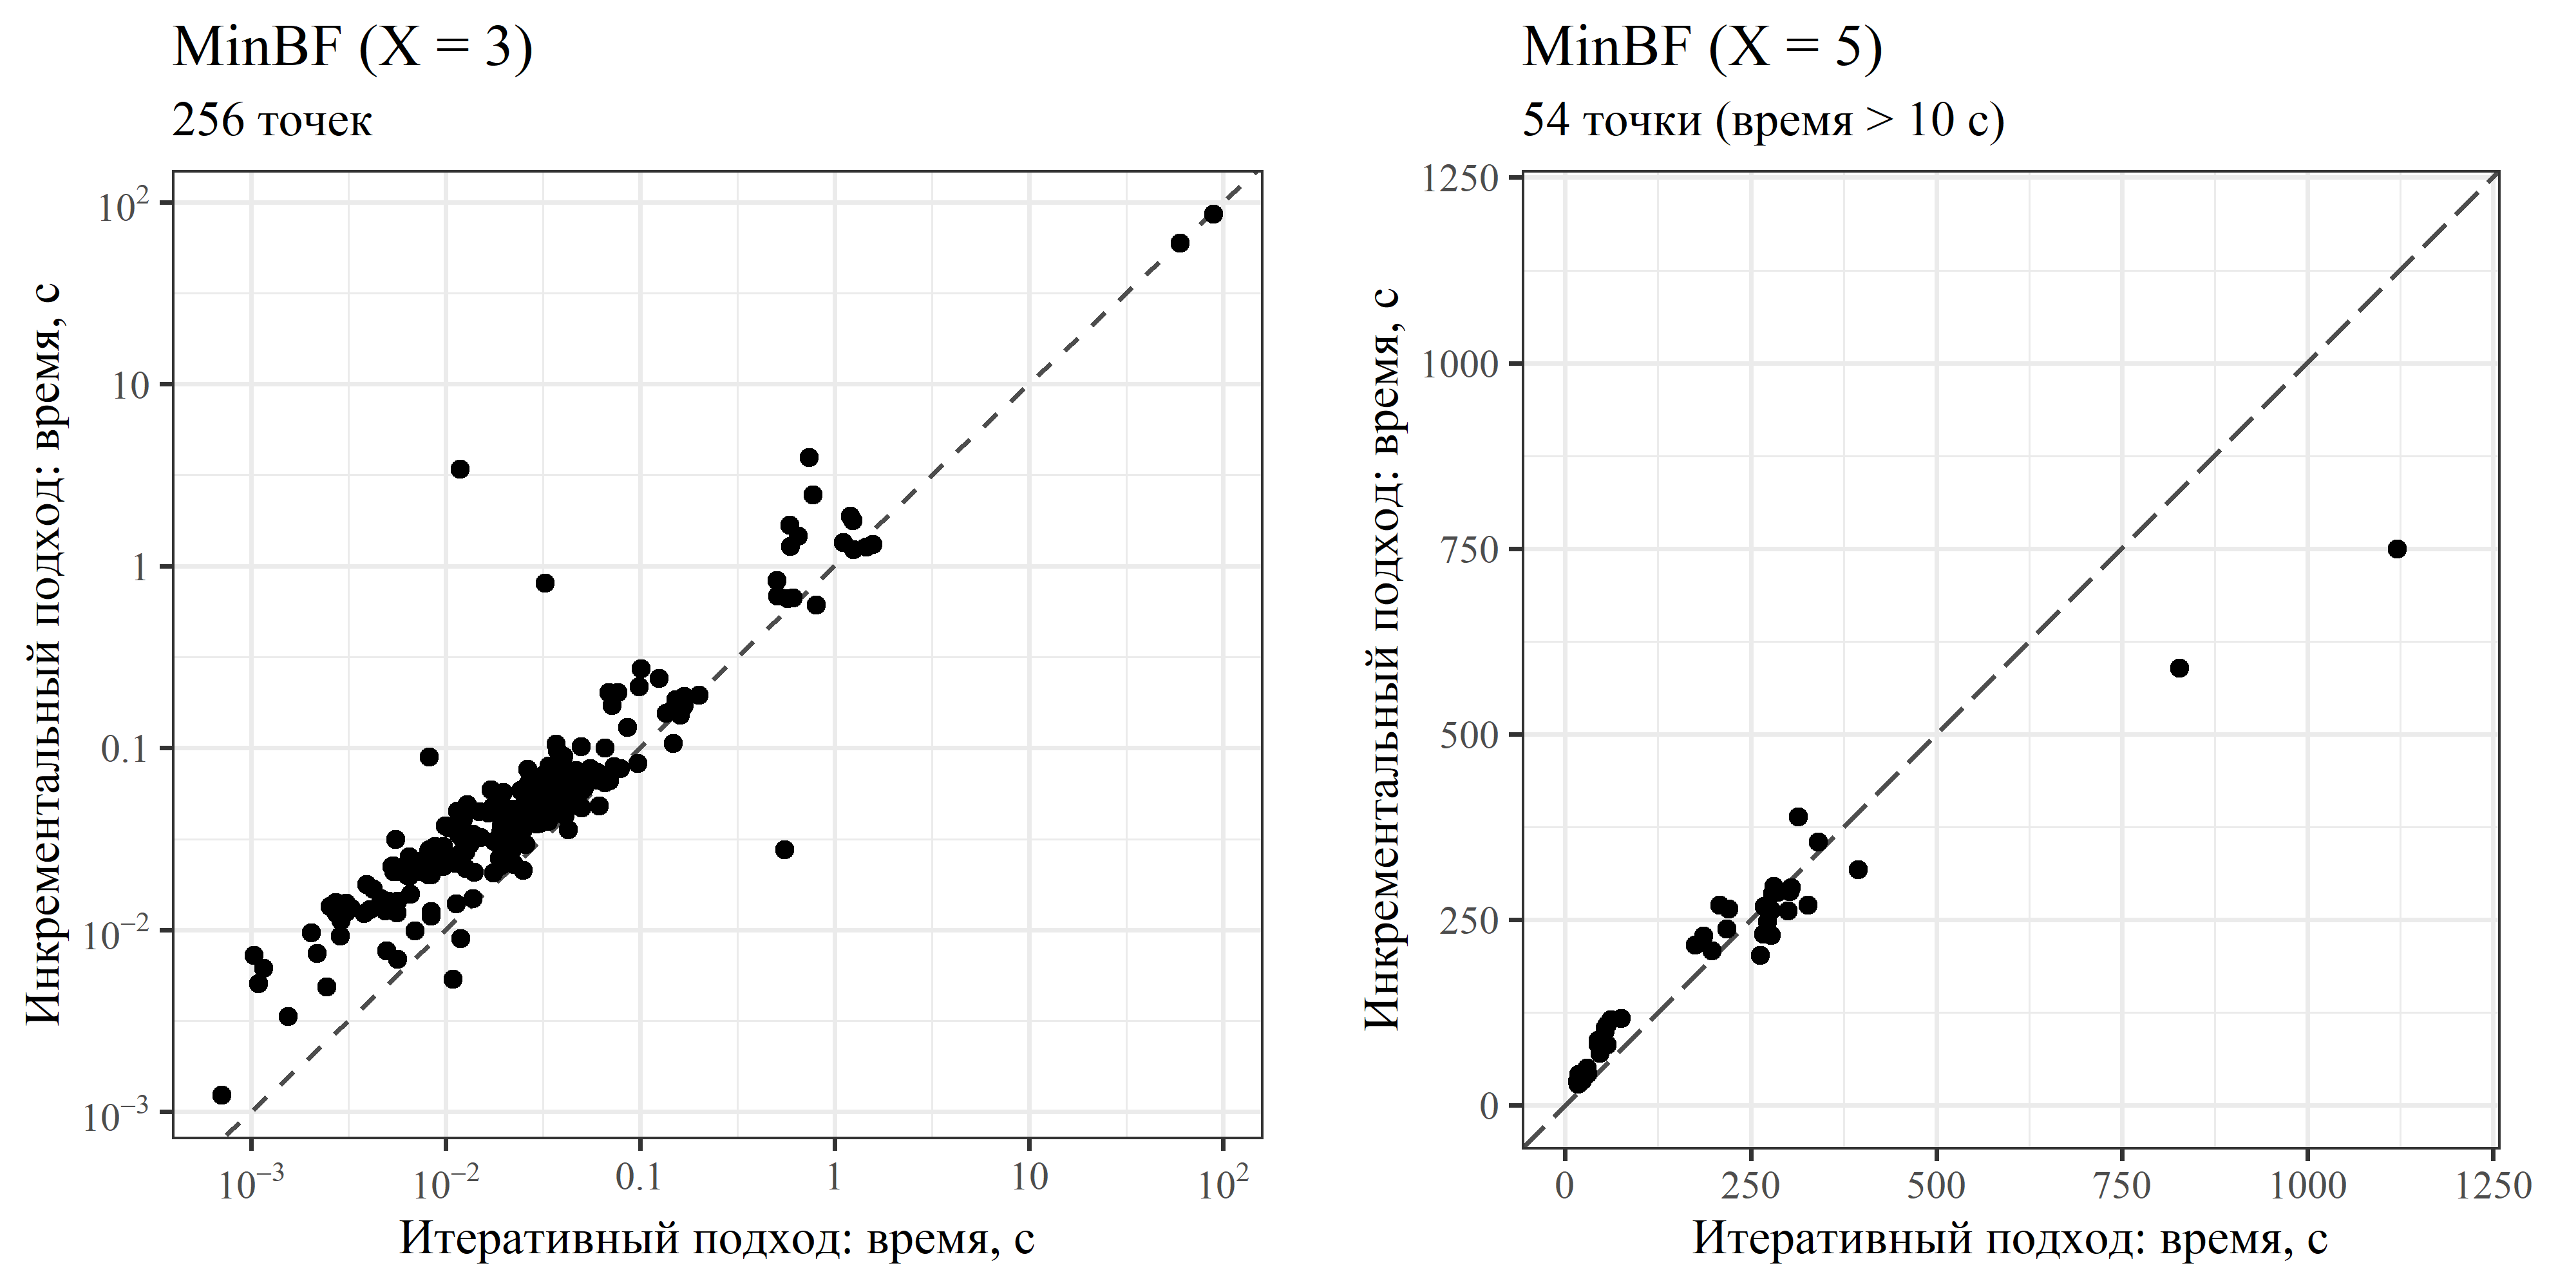
\includegraphics[max width=\linewidth]{minbf.png}
    \caption{Графики сравнения времени работы алгоритма синтеза минимальной булевой формулы (слева \--- от трех переменных, справа \--- от пяти переменных) для двух подходов: итеративный (горизонтальная ось) и инкрементальный (вертикальная ось). Время работы указано в секундах (слева \--- на логарифмической шкале). Каждая точка на графике соответствует булевой функции. На правом графике показаны только точки со временем работы, превышающим 10 секунд.}
    \label{fig:minbf}
\end{figure}

Можно заметить, что большинство минимальных формул для функций от трех переменных были найдены менее, чем за одну секунду \--- сравнение на таких масштабах времени в контексте решения NP-трудных задач не является целесообразным.
Поэтому были проведен дополнительный набор экспериментов на данных большей размерности и более \enquote{сложных} булевых функциях \--- от $X = 5$ переменных.
Результаты приведены на Рисунке~\ref{fig:minbf} (справа), где показаны только точки со временем работы, превышающим 10~секунд (всего 54~точки).
Данный график \--- а именно, точки в правой части графика под базовой линией \--- позволяет судить о том, что инкрементальный подход действительно обеспечивает лучшую производительность в рассмотренной задаче синтеза минимальной булевой формулы.


\section{Метод синтеза конечно-автоматных моделей по примерам поведения, основанный на сведении к SAT}%
\label{sec:automata-synthesis}

В этом разделе приводится описание разработанного метода синтеза минимальных конечно-автоматных моделей базовых функциональных блоков по примерам поведения.
Расширение метода, позволяющее также учитывать формальную спецификацию в виде LTL-формул, рассматривается в разделе~\ref{sec:cegis}.
Сначала рассматривается решение базовой задачи (алгоритм $\AlgoBasic$) \--- синтеза моделей с использованием только сценариев выполнения \--- приводится описание переменных и ограничений, составляющих сведение к задаче SAT и предлагается итеративный подход к синтезу минимальных моделей.
Следом, сведение к SAT расширяется (алгоритм $\AlgoExtended$) кодированием структуры деревьев разбора произвольных булевых формул охранных условий, что приводит к возможности учета их суммарного размера при минимизации.
В~заключение, решается задача синтеза модели, не только удовлетворяющей заданным примерам поведения, но и лишенной нежелательного поведения, выражаемого в виде негативных сценариев выполнения (алгоритм $\AlgoComplete$).
% После этого рассматривается подход индуктивного синтеза, основанного на контрпримерах (\textit{Counterexample\-/Guided Inductive Synthesis} \--- CEGIS), позволяющий решить (алгоритмы $\AlgoComplete$ и $\AlgoCegis$) поставленную задачу синтеза моделей одновременно по сценариям выполнения и LTL\-/спецификации.
% Разработанные методы реализованы в виде программного средства \smallcaps{fbSAT}~\cite{fbSAT-tool}.


\subsection{Кодирование структуры автомата}%
\label{sub:encoding-automaton-structure}

Сведение обозначенной задачи синтеза к задаче SAT заключается в построении булевой формулы, которая истина тогда и только тогда, когда существует конечный автомат размера $\card{\SetStates} = C$, удовлетворяющий заданному набору позитивных сценариев выполнения $\SetPositiveScenarios$.
Для этого необходимо рассмотреть процесс проверки соответствия автомата дереву сценариев и закодировать его в SAT\footnotemark.
\footnotetext{Здесь и далее фраза \enquote{закодировать в SAT} означает построение соответствующей булевой формулы в КНФ, кодирующей структуру и требуемые ограничения задачи синтеза.}
При этом также необходимо закодировать структуру синтезируемого объекта \--- конечного автомата, а точнее, ECC\@.
Здесь и далее в этом разделе предполагается, что $b \in \Bool = \Set{\top, \bot}$, $q \in \SetStates$, $k \in [1..K]$, $e \in \SetInputEvents$, $u \in \SetTreeInputs$, $v \in \SetTreeNodes$, если не указано иное.

Искомый автомат состоит из $C$ состояний, каждое из которых имеет ассоциированное \textit{действие} (выходное событие и алгоритм) и не более $K$ выходящих (\textit{outgoing}) переходов, упорядоченных в порядке их приоритета.
Выходное событие состояния $q \in \SetStates$ кодируется с помощью переменной $\StateOutputEvent_{q} \in \SetOutputEvents \union \Set{\varepsilon}$.
% \footnote{Здесь и далее под кодирующей переменной подразумевается либо непосредственно булева переменная, либо набор булевых переменных, соответствующих значениям переменной с ограниченным доменом (например, при кодировании целочисленной переменной $x \in \Set{1,2,3}$ объявляются булевы переменные $x_1, x_2, x_3$}
Так как алгоритм является функцией, независимо изменяющей значения выходных переменных, то он кодируется с помощью переменной $\StateAlgorithm_{q,z,b} \in \Bool$, где
$q \in \SetStates$ \--- состояние автомата,
$z \in \SetOutputVariables$ \--- выходная переменная,
$b \in \Bool$ \--- текущее значение выходной переменной.
Каждый переход в автомате ассоциирован с \textit{охранным условием} \--- парой из входного события и булевой формулы, зависящей от входных переменных $\SetInputVariables$ соответствующего базового функционального блока.
Переменная~$\TransitionDestination_{q,k} \in \SetStatesAux = \SetStates \union \{ q_0 \}$ кодирует конец $k$-го перехода из состояния~$q \in \SetStates$.
\enquote{Переходы} в фиктивное состояние~$q_0$ называются \textit{нулевыми} (\textit{null-transitions}) и означают отсутствие перехода в автомате.
Входное событие на переходе кодируется с помощью переменной $\TransitionInputEvent_{q,k} \in \SetInputEvents \union \Set{\varepsilon}$.
Так как каждый переход должен обладать входным событием, то $\varepsilon$-событием отмечены только \textit{нулевые} (несуществующие) переходы: $(\TransitionDestination_{q,k} = q_0) \iff (\TransitionInputEvent_{q,k} = \varepsilon)$.
Переменная $\TransitionFiring_{q,k,e,u} \in \Bool$ кодирует функцию активации охранного условия \--- выполнение перехода при входном действии~$\Action{e}{u}$.
Переменная $\TransitionTruthTable_{q,k,u} \in \Bool$ кодирует таблицу истинности охранного условия \--- значения соответствующей булевой функции на входах~$u \in \SetTreeInputs$.
Взаимосвязь между этими переменная задается следующим образом:
\[
    \TransitionFiring_{q,k,e,u}
    \iff
    \Bigl(
        (\TransitionInputEvent_{q,k} = e)
        \land
        \TransitionTruthTable_{q,k,u}
    \Bigr) %.
\]

В соответствии со стандартом IEC~61499, переходы ECC обладают приоритетом.
Переменная $\TransitionFirstFired_{q,e,u} \in [0..K]$ кодирует индекс перехода, который выполняется \textit{первым} при входном действии $\Action{e}{u}$ \=== только этот переход будет учтен в момент исполнения ECC, даже если следующие переходы также выполняются.
При этом $\TransitionFirstFired_{q,e,u} = 0$ означает, что \emph{ни один} переход не выполняется при входном действии~$\Action{e}{u}$.
Некоторый $k$-й переход выполняется \emph{первым} тогда и только тогда, когда (1)~он выполняется ($\TransitionFiring_{q,k,e,u} = \top$) и (2)~не выполняются все предыдущие ($k' < k$) переходы.
Наивный способ кодирования переменной~$\TransitionFirstFired$ выглядит следующим образом:
\[
    (\TransitionFirstFired_{q,e,u} = k)
    \iff
    \Bigl(
        \TransitionFiring_{q,k,e,u}
        \land
        \bigland_{\mathclap{1 \leq k' < k}}
        \neg\TransitionFiring_{q,k',e,u}
    \Bigr) %.
\]
Более эффективный способ кодирования заключается в определении специальной переменной~$\TransitionNotFired_{q,k,e,u} \in \Bool$ для кодирования того факта, что все переходы с~1 по~$k$-й не выполняются.
При этом можно заметить, что такая переменная может быть определена рекурсивно:
\[
    \TransitionNotFired_{q,k,e,u}
    \iff
    \Bigl(
        \neg\TransitionFiring_{q,k,e,u}
        \land
        \TransitionNotFired_{q,k-1,e,u}
    \Bigr) ,
\]
где следует считать, что $\TransitionNotFired_{q,0,e,u} = \bot$.
Исходя из этого, эффективный способ кодирования переменной~$\TransitionFirstFired$ выглядит следующим образом:
\[
    (\TransitionFirstFired_{q,e,u} = k)
    \iff
    \left(
        \TransitionFiring_{q,k,e,u}
        \land
        \TransitionNotFired_{q,k-1,e,u}
    \right) %.
\]


% TODO: ограничения

Рассмотрим сценарий выполнения $s \in \SetPositiveScenarios$ и автомат~$\Automaton$, изначально находящийся в стартовом состоянии~$\InitialState$.
Автомат последовательно обрабатывает входные действия из сценария и, возможно (если выполняется какой-либо переход \--- соответствующее охранное условие становится истинным), изменяет состояние, продуцируя выходные действия.
Когда автомат находится в состоянии~$q$ и обрабатывает входное действие~$\InputAction$, он либо (1)~переходит в состояние~$q'$, либо (2)~\enquote{игнорирует} входное действие, оставаясь в том же состоянии.
Такое поведение описывается переменной $\ActualTransitionFunction_{q,e,u} \in \SetStatesAux$, где $\ActualTransitionFunction_{q,e,u} = q_0$ соответствует второму~(2) случаю.
Заметим, что в первом случае автомат может перейти по переходу-петле и остаться в исходном состоянии $q' = q$, что, однако, отличается от случая $q' = q_0$, при котором не происходит генерации выходного действия, ассоциированного с состоянием~$q$.


\subsection{BFS-предикаты нарушения симметрии для состояний автомата}%
\label{sub:encoding-bfs-automaton}

Дополнительно, стоит добавить ограничения нарушения симметрии (\textit{symmetry breaking predicates})~\cite{ulyantsev2015}, форсирующие нумерацию состояний автомата в порядке BFS-обхода (\textit{breadth-first search}) \--- в том порядке, в котором они были бы посещены при выполнении поиска в ширину из стартового состояния.
Такие ограничения позволяют существенно сократить пространство поиска, что позитивно влияет на время решения задачи SAT.
Стоит отметить, что данные ограничения не влияют на корректность решения \--- если решение существует, то оно будет найдено независимо от нумерации состояний автомата.

Суть BFS-предиката нарушения симметрии заключается в следующем наблюдении относительно дерева BFS-обхода: родителем каждой вершины может быть только вершина с меньшим номером, а потомки каждой вершины следуют в строгом возрастающем порядке \--- номера соседних (\textit{sibling}) вершин отличаются на~1.
Из~этого следует, что для каждой вершины $i > 1$ верно следующее: родитель соседней ($i + 1$) вершины либо совпадает с родителем вершины~$i$, либо имеет больший номер.
Для кодирования такого ограничения в SAT, необходимо объявить следующие переменные.
Переменная $\BfsTransitionAutomaton_{q_i,q_j} \in \Bool$ ($q_i,q_j \in \SetStates$) кодирует наличие любого перехода из~$q_i$ в~$q_j$ в автомате:
\[
    \BfsTransitionAutomaton_{q_i,q_j}
    \iff
    \biglorclap{k \in [1..K]}
    (\TransitionDestination_{q_i,k} = q_j) %.
\]
Переменная $\BfsParentAutomaton_{q_j} \in \Set{q_1,\dotsc,q_{j-1}}$ ($q_j \in \SetStates$) кодирует родителя вершины~$q_j$ в дереве BFS-обхода:
\[
    (\BfsParentAutomaton_{q_j} = q_i)
    \iff
    \Bigl(
        \BfsTransitionAutomaton_{q_i,q_j}
        \land
        \bigland_{\mathclap{r < i}}
        \neg \BfsTransitionAutomaton_{q_r,q_j}
    \Bigr) %.
\]
Непосредственно BFS-ограничение выглядит следующим образом:
\[
    (\BfsParentAutomaton_{q_j} = q_i)
    \implies
    (\BfsParentAutomaton_{q_{j+1}} \geq q_i) %.
\]

Можно заметить, что в BFS-ограничении присутствует отношение $(\BfsParentAutomaton_{q_{j+1}} \geq q_i)$.
Наивный способ кодирования такого ограничения в SAT выглядит следующим образом:
\[
    (\BfsParentAutomaton_{q_j} = q_i)
    \implies
    \bigland_{\mathclap{r < i}}
    (\BfsParentAutomaton_{q_{j+1}} \neq q_r) %.
\]
Однако существуют и другие, теоретически более эффективные способы.
Например, можно использовать так называемые \enquote{переменные, кодирующие порядок} (\textit{order-encoding})~\cite{order-encoding}.
Перед тем, как перейти к их описанию, необходимо напомнить, что привычные переменные с ограниченным доменом, например, $x \in \Set{2, 3, 5}$, кодируются следующим образом, называемым в разных источниках как \enquote{\textit{onehot}}, \enquote{\textit{sparse encoding}}, \enquote{\textit{direct encoding}}~\cite{direct-encoding}, \enquote{\textit{pairwise encoding}}: для каждого значения из домена создается отдельная булева переменная, кодирующая равенство переменной этому значению, например, $x \mathrel{\mathord{\bowtie}_{\mathit{onehot}}} \Set{x_2, x_3, x_5}$, где $x_2 \equiv (x = 2)$, $x_3 \equiv (x = 3)$, $x_5 \equiv (x = 5)$.
Аналогичным образом определяются и \textit{order-encoded} переменные, однако кодируют они не равенство, а отношение порядка, например, $x \mathrel{\mathord{\bowtie}_{\mathit{order}}} \Set{x'_2, x'_3, x'_4, x'_5}$, где $x'_i \equiv (x \geq i)$.
Заметим, что на практике домены переменных являются непрерывными\footnote{Под \enquote{непрерывным} доменом здесь подразумевается дискретная последовательность без \enquote{пропусков}, что в случае численных доменов выражается в виде интервала $[\text{low}..\text{high}]$.}, поэтому кодирующих переменных будет столько же, сколько и при \textit{onehot}-кодировании\footnote{Можно заметить, что в рассмотренном примере переменная $x'_2 \equiv (x \geq 2)$ всегда истинна, а значит ее можно не вводить, поэтому корректнее говорить, что \textit{order-encoded} переменных всегда на одну меньше \textit{onehot}.}.
Детальное описание \textit{order encoding} присутствует в~\cite{order-encoding} и в данной работе не приводится.
Таким образом, BFS-предикат с использованием \textit{order-encoded} переменной $\BfsParentAutomatonOrder_{q_j} \equiv (\BfsParentAutomaton_{q_j} \geq q_j)$ может быть сформулирован следующим образом:
\[
    (\BfsParentAutomaton_{q_j} = q_i)
    \implies
    \BfsParentAutomatonOrder_{q_i}
\]
К сожалению, данное усовершенствование не привело к видимым изменениям производительности сведения (результаты экспериментального исследования не приводятся), поэтому здесь и далее в данной работе считается, что используется наивный способ кодирования BFS-предиката нарушения симметрии.


\subsection{Кодирование отображения позитивного дерева сценариев}%
\label{sub:encoding-positive-mapping}

%% Picture: Tree-to-automaton mapping
\begin{figure}
    \centering
    \begin{adjustbox}{max width=\linewidth}
        \subfile{tex/tikz-mapping}
    \end{adjustbox}
    \caption{Пример отображения дерева сценариев на автомат}
    \label{fig:tree-automaton-mapping}
\end{figure}

Для обеспечения соответствия автомата дереву сценариев, необходимо построить отображение $\Mapping \colon \SetTreeNodes \to \SetStates$ вершин дерева на состояния автомата.
Пример такого отображения приведен на рисунке~\ref{fig:tree-automaton-mapping}.
Переменная~$\Mapping_{v} \in \SetStates$ кодирует \textit{удовлетворяющее состояние}, в котором автомат оказывается после обработки вершины дерева~$v \in \SetTreeNodes$.
Корень дерева $\TreeRoot$ отображается в стартовое состояние автомата: $\Mapping_{\TreeRoot} = \InitialState$.
Пассивные вершины ($\toe{v} = \varepsilon$) соответствуют ситуации, когда автомат должен проигнорировать входное действие, не изменяя своего состояния, что может быть выражено с помощью следующих ограничений: $\Mapping_{v} = \Mapping_{p}$ и $\ActualTransitionFunction_{q,e,u} = q_0$, где $v \in \SetTreeNodesPassive$, $p = \tp{v}$, $q = \Mapping_{p}$, $e = \tie{v}$, $u = \tin{v}$.
Активные вершины ($\toe{v} \neq \varepsilon$) соответствуют ситуации, когда автомат должен отреагировать на входное действие и продуцировать определенное (непустое) выходное действие, что может быть закодировано следующим образом:
\[
    (\Mapping_{v} = q')
    \implies
    \Bigl(
        (\ActualTransitionFunction_{q,e,u} = q')
        \land
        (\StateOutputEvent_{q'} = o)
        \land
        \bigland_{\mathclap{z \in Z}}
        (\StateAlgorithm_{q',z,b} = b')
    \Bigr),
\]
где
$v \in \SetTreeNodesActive$,
$p = \tp{v}$,
$q = \Mapping_{p}$,
$q' \in \SetStates$,
$e = \tie{v}$,
$u = \tin{v}$,
$o = \toe{v}$,
$z \in Z$,
$b = \tov{p,z}$,
$b' = \tov{v,z}$.


\subsection{Кодирование ограничений на количество переходов}%
\label{sub:encoding-transitions-bounds}

Для того, чтобы ограничить количество переходов в автомате \--- закодировать ограничение вида \enquote{суммарное число \emph{ненулевых} переходов в автомате не больше~$T$}, можно воспользоваться техникой \textit{totalizer} (раздел~\ref{sec:cardinality}) и закодировать в SAT \textit{ограничение на кардинальность}~$\Phi(\mathcal{D}, 0, T)$, где $\mathcal{D} = \Set{ \TransitionDestination_{q,k} \neq q_0 \given q \in \SetStates, k \in [1..K] }$ \--- множество интересующих переменных, $T$ \=== верхняя граница для суммарного числа ненулевых переходов в автомате.
Стоит отметить, что на практике интерес представляет задача минимизации числа переходов в автомате, рассматриваемая в данной работе далее, поэтому нижняя граница принимается равной нулю.
Техника \textit{totalizer} позволяет кодировать сразу две границы, что может быть полезно при иных постановках задачи \--- например, возможно синтезировать автомат с точным (заранее известным) числом переходов~$T^{*}$, для чего необходимо закодировать обе границы, равные~$T^{*}$ \--- однако такие задачи в данной работе не рассматриваются.


\subsection{Алгоритм \AlgoBasic}%
\label{sub:algorithm-basic}

Описанные выше переменные и ограничения позволяют синтезировать \emph{вычислимые} конечно-автоматные модели \--- модели, способные реагировать на входные воздействия, генерируя выходные действия.
Обозначим $\AlgoBasicFull(\SetPositiveScenarios, C,\nobreak T)$ процедуру нахождения автомата, который удовлетворяет заданному набору позитивных сценариев выполнения~$\SetPositiveScenarios$, и в котором~$C$ состояний и суммарно не более~$T$ переходов.
Данная процедура состоит из (1)~построения позитивного дерева сценариев~$\PositiveTree$, (2)~формирования сведения к SAT (кодирование структуры автомата, отображения дерева сценариев и ограничения на кардинальность) и (3)~вызова SAT-решателя.
Результатом работы данной процедуры является либо искомый конечный автомат, либо доказательство отсутствия автомата заданного размера.
Также введем обозначение для случая, когда число переходов в автомате остается неограниченным:
\[
    \AlgoBasic(\SetPositiveScenarios, C) = \AlgoBasicFull(\SetPositiveScenarios, C, {T = \infty})
\]
Стоит отметить, что параметр~$K$ \--- максимальное число переходов из каждого состояния \--- здесь и далее принимается равным $K = C \cdot \card{\SetInputEvents}$, так как при меньших значениях возможно отсутствие решения из-за слишком сильных ограничений на искомую модель, а~дополнительный перебор подходящего значения~$K$ является обременительной задачей.
% Также стоит отметить, что уменьшение параметра~$K$ значительно сокращает размер сведение, а значит, увеличивает эффективность решения задачи синтеза, поэтому любые оценки данного параметра могут быть исключительно полезны.


\subsection{Кодирование структуры охранных условий}%
\label{sub:encoding-guards-structure}

В описанном выше сведении охранные условия представляются в виде таблиц истинности соответствующих булевых формул \--- посредством переменной~$\TransitionTruthTable$.
Однако такие охранные условия сложны для восприятия человеком, а также неприменимы в средствах разработки систем управления, таких так Matlab или nxtSTUDIO~\cite{nxtstudio}, где охранные условия должны быть явно представлены в виде булевых формул.
Поэтому сведение расширяется кодированием деревьев разбора произвольных булевых формул, зависящих от входных переменных $\SetInputVariables$.

Каждое дерево разбора охранного условия на $k$-м переходе (${k \in [1..K]}$) из состоянияЁ$q \in \SetStates$ состоит из $P$ вершин, где~$P$ является параметром разрабатываемого метода.
Каждая вершина типизирована и может быть либо булевым оператором, либо терминальной вершиной, соответствующей входной переменной.
Здесь стоит отметить, что параметр~$P$ является \enquote{глобальным} для всего автомата \--- \emph{все} охранные условия состоят из $P$ вершин.
Так как существуют булевы формулы, для записи которых достаточно менее~$P$ вершин в дереве разбора, некоторые вершины могут быть \enquote{нетипизированными} (\textit{none-typed}) \--- не включаться в дерево.
Размер дерева разбора определяется как число \textit{типизированных} вершин в нем.
Здесь и далее будут использованы следующие обозначения, если не указано иное: ${p \in [1..P]}$, ${x \in \SetInputVariables}$, ${u \in \SetTreeInputs}$.

Переменная $\NodeType_{q,k,p} \in \Set{\NodeTypeTerminal, \NodeTypeAnd, \NodeTypeOr, \NodeTypeNot, \NodeTypeNone}$ кодирует тип вершины дерева разбора~$p$, где \enquote{$\NodeTypeTerminal$}~обозначает терминальные вершины, \enquote{$\NodeTypeAnd$}, \enquote{$\NodeTypeOr$}, \enquote{$\NodeTypeNot$} \--- логические операторы, а \enquote{$\NodeTypeNone$} \--- нетипизированные вершины.
Без потери общности можно задать ограничение на то, что нетипизированные вершины имеют наибольшие номера в дереве:
\[
    (\NodeType_{q,k,p} = \NodeTypeNone)
    \implies
    (\NodeType_{q,k,p+1} = \NodeTypeNone) %.
\]
Переменная~$\NodeInputVariable_{q,k,p} \in {\SetInputVariables \union \Set{0}}$ кодирует входную переменную, ассоциированную с терминальной вершиной~$p$, или ее отсутствие ($\NodeInputVariable_{q,k,p} = 0$).
Только терминальные вершины могут иметь ассоциированные входные переменные:
\[
    (\NodeType_{q,k,p} = \NodeTypeTerminal)
    \iff
    (\NodeInputVariable_{q,k,p} \neq 0)
\]

Для задания структуры дерева разбора, а именно, для определения родительских связей между вершинами, используются переменные $\NodeParent_{q,k,p} \in [0..(p-1)]$ и~$\NodeChild_{q,k,p} \in \Set{0} \union [(p+1)..P]$, кодирующие, соответственно, родителя и \emph{левого} ребенка вершины~$p$ (либо их отсутствие: $\NodeParent_{q,k,p} = 0$, $\NodeChild_{q,k,p} = 0$).
Взаимосвязь между этими переменными задается следующим образом:
\[
    (\NodeChild_{q,k,p} = ch)
    \implies
    (\NodeParent_{q,k,ch} = p)
\]
Только типизированные вершины, кроме корня ($p = 1$), имеют родительские вершины:
\[
    (\NodeParent_{q,k,p} \neq 0)
    \iff
    (\NodeType_{q,k,p} \neq \NodeTypeNone)
\]
Стоит отметить, что правый ребенок вершины дерева разбора не кодируется явно \--- для бинарных операторов предполагается, что он имеет номер на единицу больше левого ребенка ($c \in\nobreak [(p+1)..(P-1)]$):
\[
    \Bigl(
        (\NodeType_{q,k,p} \in \{ \NodeTypeAnd, \NodeTypeOr \})
        \land
        (\NodeChild_{q,k,p} = c)
    \Bigr)
    \implies
    (\NodeParent_{q,k,c+1} = p) %.
\]

Переменная $\NodeValue_{q,k,p,u} \in \Bool$ кодирует значение подформулы \--- булевого выражения, соответствующего поддереву с корнем~$p$ \--- на входе~$u$.
Значение корня дерева разбора соответствует значению всей булевой формулы охранного условия, а значит, можно переиспользовать переменную~$\TransitionTruthTable_{q,k,u}$, объявленную ранее:
\[
    \TransitionTruthTable_{q,k,u}
    \equiv
    \NodeValue_{q,k,1,u} %.
\]
Значения терминальных вершин соответствуют значениям ассоциированных входных переменных;
значения вершин-операторов могут быть вычислены на основе значений вершин-потомков;
значения нетипизированных вершин для определенности принимаются равными \texttt{False}, однако это является лишь технической деталью реализации \--- значения нетипизированных вершин впоследствии не используются:
\begin{align*}
    \Bigl(
        (\NodeType_{q,k,p} = \NodeTypeTerminal)
        \land
        (\NodeInputVariable_{q,k,p} = x)
    \Bigr)
    &\implies
    \bigland_{\mathclap{u \in \SetTreeInputs}}
    \left[
        \NodeValue_{q,k,p,u}
        \iff
        u_x
    \right]
\\
    \Bigl(
        (\NodeType_{q,k,p} = \NodeTypeAnd)
        \land
        (\NodeChild_{q,k,p} = c)
    \Bigr)
    &\implies
    \bigland_{\mathclap{u \in \SetTreeInputs}}
    \left[
        \NodeValue_{q,k,p,u}
        \iff
        (\NodeValue_{q,k,c,u} \land \NodeValue_{q,k,c+1,u})
    \right]
\\
    \Bigl(
        (\NodeType_{q,k,p} = \NodeTypeOr)
        \land
        (\NodeChild_{q,k,p} = c)
    \Bigr)
    &\implies
    \bigland_{\mathclap{u \in \SetTreeInputs}}
    \left[
        \NodeValue_{q,k,p,u}
        \iff
        (\NodeValue_{q,k,c,u} \lor \NodeValue_{q,k,c+1,u})
    \right]
\\
    \Bigl(
        (\NodeType_{q,k,p} = \NodeTypeNot)
        \land
        (\NodeChild_{q,k,p} = c)
    \Bigr)
    &\implies
    \bigland_{\mathclap{u \in \SetTreeInputs}}
    \left[
        \NodeValue_{q,k,p,u}
        \iff
        \neg\NodeValue_{q,k,c,u}
    \right]
\\
    (\NodeType_{q,k,p} = \NodeTypeNone)
    &\implies
    \bigland_{\mathclap{u \in \SetTreeInputs}}
    \neg\NodeValue_{q,k,p,u}
    %.
\end{align*}


\subsection{BFS-предикаты нарушения симметрии для охранных условий}%
\label{sub:encoding-bfs-guards}

Дополнительно, стоит добавить ограничения нарушения симметрии, форсирующие BFS-нумерацию вершин дерева разбора охранного условия.
Фактически, они аналогичны BFS-ограничениям для состояний автомата (раздел~\ref{sub:encoding-bfs-automaton}), но применяются не ко всему автомату, а к каждому дереву разбора охранного условия по-отдельности: для каждого $q \in \SetStates$, $k \in [1..K]$.
Переменная $\BfsTransitionGuard_{i,j} \in \Bool$ (${1 \leq i < j \leq P}$) задает существование \enquote{перехода} из $i$-ой вершины в~$j$-ую:
\[
    \BfsTransitionGuard_{i,j}
    \iff
    (\NodeParent_{q,k,j} = i) %.
\]
Переменная $\BfsParentGuard_{j} \in [1..(j-1)]$ ($j \in [2..P]$) кодирует родителя $j$-й вершины в дереве BFS-обхода:
\[
    (\BfsParentGuard_{j} = i)
    \iff
    \Bigl(
        \BfsTransitionGuard_{i,j}
        \land
        \bigland_{\mathclap{r < i}}
        \neg \BfsTransitionGuard_{r,j}
    \Bigr) %.
\]
Непосредственно BFS-ограничение задается следующим образом:
\[
    (\BfsParentGuard_{j} = i)
    \implies
    % just relation?
    \bigland_{\mathclap{r < i}}
    (\BfsParentGuard_{j+1} \neq r) %.
\]


\subsection{Кодирование ограничений на суммарный размер охранных условий}%
\label{sub:encoding-guards-bounds}

Для того, чтобы ограничить размер охранных условий в автомате, то есть закодировать ограничение вида \enquote{суммарное число \textit{типизированных} вершин в деревьях разбора булевых формул, соответствующих охранным условиям на переходах автомата не больше~$N$}, можно воспользоваться техникой \textit{totalizer} (см.~раздел~\ref{sec:cardinality}) и закодировать в SAT \textit{ограничение на кардинальность}~$\Phi(\mathcal{H}, 0, N)$, где $\mathcal{H} = \Set{ \NodeType_{q,k,p} \neq\nobreak \NodeTypeNone \given q \in \SetStates, k \in [1..K], p \in [1..P] }$ \--- множество интересующих переменных, $N$ \=== верхняя граница для суммарного размера охранных условий в автомате.


\subsection{Алгоритм \AlgoExtended}%
\label{sub:algorithm-extended}

Обозначим $\AlgoExtendedFull(\SetPositiveScenarios, C, P, N)$ процедуру нахождения автомата, который удовлетворяет заданному набору позитивных сценариев выполнения~$\SetPositiveScenarios$, и в котором~$C$ состояний, максимальный размер охранного условия~$P$, а суммарный размер охранных условий не больше~$N$.
Стоит отметить, что параметр~$T$ \--- число ненулевых переходов в автомате \--- здесь и далее не рассматривается.
Данная процедура состоит из (1)~построения позитивного дерева сценариев~$\PositiveTree$, (2)~формирования сведения к SAT (кодирование структуры автомата и охранных условий, отображения дерева сценариев и ограничения на кардинальность) и (3)~вызова SAT-решателя.
Также введем обозначение для случая, когда суммарный размер охранных условий в автомате остается неограниченным:
\[
    \AlgoExtended(\SetPositiveScenarios, C, P) = \AlgoExtendedFull(\SetPositiveScenarios, C, P, N=\infty)
\]
Стоит отметить, что минимизация параметра~$T$ \--- числа \textit{ненулевых} переходов в автомате \--- в данном случае не производится, потому что если сначала минимизировать~$T$, а затем~$N$, то полученное решение не будет наименьшим, а если наоборот \--- сначала~$N$, а затем~$T$ \--- то это не повлияет на уже полученное минимальное значение~$\Nmin$.


\subsection{Кодирование отображения негативного дерева сценариев}%
\label{sub:encoding-negative-mapping}

Отображение $\NegativeMapping \colon \SetNegativeTreeNodes \to \SetStatesAux$ вершин негативного дерева сценариев~$\NegativeTree$ на состояния автомата очень похоже на отображение позитивного дерева, однако главным отличием является то, что негативное дерево представляет нежелательное поведение системы, включая нежелательное циклическое поведение, которое необходимо запретить.

Переменная $\NegativeMapping_{\negv} \in \SetStatesAux$ кодирует \textit{удовлетворяющее} состояние (либо его отсутствие: $\NegativeMapping_{\negv} = q_0$).
Стоит отметить, что автомат может не обладать поведением, заданным в негативном дереве сценариев \--- его поведение может отличаться от записанного в вершине дерева $\negv \in \SetNegativeTreeNodes$ \--- в этом (и только в этом) случае $\NegativeMapping_{\negv} = q_0$.
Eсли некоторая вершина $\negv \in \SetNegativeTreeNodes$ никуда не отображается (отображается в \enquote{фиктивное} состояние~$q_0$), то это распространяется далее через потомков:
\[
    (\NegativeMapping_{\negtp{\negv}} = q_0)
    \implies
    (\NegativeMapping_{\negv} = q_0) %.
\]
Корень негативного дерева~$\NegativeTreeRoot$ отображается в стартовое состояние автомата:
\[
    \NegativeMapping_{\NegativeTreeRoot} = \InitialState %.
\]

Пассивные вершины дерева сценариев описывают поведение, когда автомат игнорирует входное действие и не изменяет своего состояния, значит, если автомат соответствует такому поведению, то пассивная вершина отображается \--- аналогично позитивному дереву \--- в то же состояние, что и ее родитель, иначе же вершина никуда не отображается: \(
    (\NegativeMapping_{\negv} = \NegativeMapping_{\negtp{\negv}})
    \lor
    (\NegativeMapping_{\negv} = q_0)
\),
где $\negv \in \SetNegativeTreeNodesPassive$.

В свою очередь активные вершины дерева сценариев описывают поведение, когда автомат должен отреагировать на входное воздействие определенным образом, значит, если автомат соответствует такому поведению, то отображение активной вершины аналогично позитивному дереву, иначе же вершина никуда не отображается:
\[
    (\NegativeMapping_{\negv} = q')
    \iff
    \Bigl(
        (\NegativeActualTransitionFunction_{q,e,u} = q')
        \land
        (\StateOutputEvent_{q'} = o)
        \land
        \bigland_{\mathclap{z \in \SetOutputVariables}}
        (\StateAlgorithm_{q',z,b} = b')
    \Bigr) ,
\]
где
$\negv \in \SetNegativeTreeNodesActive$,
$\Negative{p} = \negtp{\negv}$,
$q = \NegativeMapping_{\Negative{p}}$,
$q' \in \SetStates$,
$e = \negtie{\negv}$,
$u = \negtin{\negv}$,
$o = \negtoe{\negv}$,
$z \in \SetOutputVariables$,
$b = \negtov{\Negative{p},z}$,
$b' = \negtov{\negv,z}$.
Стоит отметить, что в этом ограничении используется эквивалентность (\enquote{$\iff$}), а не импликация (\enquote{$\implies$}), что позволяет не рассматривать отдельно определение для случая $q' = q_0$, при котором было бы необходимо учитывать различные варианты несоответствия поведения автомата поведению, записанному в вершине негативного дерева.

В заключение, необходимо запретить в автомате нежелательное циклическое поведение, представляемое с помощью \emph{обратных ребер}.
Для этого необходимо, чтобы вершины негативного дерева, являющиеся началом и концом обратного ребра, отображались в различные состояния, либо же не отображались вовсе:
\[
    \bigland_{\vphantom{\widehat{V}} \negv \in \SetNegativeTreeNodes}
    \;
    \bigland_{\vphantom{\widehat{V}} \negv' \in \negtbe{\negv}}
    \Bigl[
        (\NegativeMapping_{\negv} \neq \NegativeMapping_{\negv'})
        \lor
        (\NegativeMapping_{\negv} = \NegativeMapping_{\negv'} = q_0)
    \Bigr] %.
\]


\subsection{Алгоритм \AlgoComplete}%
\label{sub:algorithm-complete}

Обозначим $\AlgoCompleteFull(\SetPositiveScenarios, \SetNegativeScenarios, C, P,\nobreak N)$ процедуру нахождения автомата, который удовлетворяет заданному набору позитивных сценариев выполнения~$\SetPositiveScenarios$ и не удовлетворяет набору негативных сценариев~$\SetNegativeScenarios$, и в котором~$C$ состояний, максимальный размер охранного условия~$P$, а суммарный размер охранных условий не больше~$N$.
Данная процедура состоит из (1)~построения позитивного дерева сценариев~$\PositiveTree$ и негативного дерева сценариев~$\NegativeTree$, (2)~формирования сведения к SAT (кодирование структуры автомата и охранных условий, отображения позитивного и негативного дерева сценариев, а также ограничения на кардинальность) и (3)~вызова SAT-решателя.
Также введем обозначение для случая, когда суммарный размер охранных условий в автомате остается неограниченным:
\[
    \AlgoComplete(\SetPositiveScenarios, \SetNegativeScenarios, C, P) = \AlgoCompleteFull(\SetPositiveScenarios, \SetNegativeScenarios, C, P, {N = \infty})
\]


\section{Синтез минимальных конечно-автоматных моделей}%
\label{sec:synth-minimal-models}

Разработанные в данной работе методы синтеза монолитных конечно-автоматных моделей зависят от трех параметров: число состояний автомата~$C$, максимальный размер каждого охранного условия~$P$ и суммарный размер всех охранных условий~$N$.
В реальности эти параметры неизвестны заранее, а их оценки, полученные какими-либо сторонними способами, могут быть далеки от оптимальных.
На практике гораздо большей ценностью обладают модели меньших размеров, ввиду их эффективности и простоты.
Обе задачи \--- \emph{автоматизация} поиска параметров и их \emph{минимизация} \--- могут быть решены одновременно путем применения \emph{итеративного} подхода к синтезу минимальных моделей, рассматриваемому в текущем разделе.


\subsection{Алгоритм \AlgoBasicMin}%
\label{sub:algorithm-basic-min}

Для быстрой оценки минимального числа состояний автомата, удовлетворяющего заданным сценариям выполнения $\SetPositiveScenarios$, используется алгоритм $\AlgoBasic(\SetPositiveScenarios, C)$ с итеративным перебором параметра~$C$ \enquote{снизу вверх}.
После нахождения минимального числа состояний~$\Cmin$ производится минимизация числа переходов в автомате с использованием алгоритма $\AlgoBasic^{*}(\SetPositiveScenarios, \Cmin, T)$ с итеративным перебором параметра~$T$ \enquote{сверху вниз}, начиная с синтеза неограниченной модели: ${T = \infty}$.
Псевдокод полученного алгоритма $\AlgoBasicMin(\SetPositiveScenarios)$ представлен в листинге~\ref{alg:basic-min} вместе со вспомогательными функциями $\AlgoBasicMinC$ и $\AlgoBasicMinT$, которые непосредственно выполняют минимизацию каждого параметра: $C$ и~$T$.

%% Algorithm: Basic-min
% TODO: \subfile{tex/algo-basic-min}


\subsection{Алгоритмы \AlgoExtendedMin\ и \AlgoCompleteMin}%
\label{sub:algorithm-extended-min-and-complete-min}

Пусть параметр $P$ \--- максимальный размер охранного условия в автомате \--- известен, а число состояний~$C$ оценено с помощью алгоритма $\AlgoBasicMinC$\@.
Последующая минимизация суммарного размера охранных условий в автомате производится аналогично алгоритму $\AlgoBasicMinT$: с использованием алгоритма $\AlgoExtendedFull(\SetPositiveScenarios, C, P,\nobreak N)$ путем итеративного перебора параметра~$N$ \enquote{сверху вниз}, начиная с синтеза неограниченной модели: ${N = \infty}$.
% Здесь стоит отметить, что при этом на каждой итерации фактически изменяется только \emph{компаратор}, кодирующий верхнюю границу~$N$, а ...
Псевдокод полученного алгоритма $\AlgoExtendedMin(\SetPositiveScenarios, P)$ приведен в листинге~\ref{alg:extended-min}.
Алгоритм $\AlgoCompleteMin(\SetPositiveScenarios, \SetNegativeScenarios, P)$ определяется аналогично алгоритму $\AlgoExtendedMin$:
$\SetPositiveScenarios$~и~$\SetNegativeScenarios$ \--- наборы позитивных и негативных сценариев выполнения,
$P$ \=== максимальный размер охранного условия,
внутри используется алгоритм $\AlgoCompleteFull$.

%% Algorithm: Extended-min
% TODO: \subfile{tex/algo-extended-min}

%% Algorithm: Extended-min-UB
% TODO: \subfile{tex/algo-extended-min-ub}


\subsection{Алгоритм \AlgoExtendedMinUB}%
\label{sub:algorithm-extended-min-ub}

На данном этапе возникает закономерный вопрос \--- как выбрать подходящее значение параметра~$P$?
Можно заметить, что решение задачи синтеза существует только если параметр~$P$ достаточно большой для того, чтобы охранные условия в автомате обладали достаточной выразительностью для представления желаемого поведения автомата.
Самый простой способ перебора параметра~$P$ \--- \enquote{снизу вверх}, начиная с $P = 1$, до тех пор, пока не будет найдено (с помощью алгоритма $\AlgoExtendedMinN$) решение с суммарным размером охранных условий $N = \Nmin^{*}$ для некоторого $P = P^{*}$.
Однако при этом может существовать некоторое $P' > P^{*}$, при использовании которого будет найдено еще меньшее решение: $\Nmin' < \Nmin^{*}$.
Поэтому для нахождения глобально-наименьшего автомата в терминах~$N$, необходимо продолжать поиск для $P > P^{*}$.
Однако при этом возникает вопрос: в какой момент необходимо остановить перебор параметра~$P$ и считать найденное ранее решение оптимальным?

Для ответа на этот вопрос, рассмотрим некоторый момент перебора, когда $P = P'$.
Заметим, что в лучшем случае все охранные условия в автомате имеют размер~1, кроме одного, имеющего размер~$P'$.
Также заметим, что в лучшем случае в автомате ровно $\Tmin$ переходов, где значение $\Tmin$ определено с помощью алгоритма $\AlgoBasicMinT$.
Исходя из этого, в лучшем случае суммарный размер охранных условий в автомате равен $\Nmin' = {\Tmin - 1 + P'}$.
Обозначим $\Nmin^{\text{best}}$ лучшее (наименьшее) значение, найденное в текущий момент.
Так как перебор параметра~$P$ производится с целью нахождения $\Nmin' < \Nmin^{\text{best}}$, то есть $\Tmin - 1 + P' < \Nmin^{\text{best}}$, то из этого следует, что верхняя граница для параметра $P$ есть $P' \leq \Nmin^{\text{best}} - \Tmin$.

Процесс перебора $P$ до теоретической верхней границы может потребовать значительного количества времени, поэтому предлагается следующая эвристика для ускорения этого процесса.
Рассмотрим два последовательных значения $P'$ и ${P'' = P' + 1}$, а также соответствующим им значения $\Nmin'$ и~$\Nmin''$.
Равенство ${\Nmin' = \Nmin''}$ говорит о том, что процесс поиска оптимального~$P$ находится в локальном минимуме \--- \emph{на плато}.
Если при увеличении~$P''$ равенство сохраняется, то в таком случае увеличивается \textit{ширина плато}, равная~${P'' - P'}$.
Обозначим~$w$ критическое значение ширины плато, при достижении которого останавливается перебор~$P$.
Выбор подходящего значения~$w$ обеспечивает компромисс между временем выполнения и глобальной минимальностью полученного решения.
На практике, значение~${w = 2}$ является оптимальным.
Стоит отметить, что при использовании данной эвристики разработанные методы остаются \emph{точными} \--- синтезированные автоматы так же соответствуют заданному поведению.

Обозначим $\AlgoExtendedMinUB(\SetPositiveScenarios,\nobreak w)$ процесс синтеза минимальной модели, удовлетворяющей заданным сценариям выполнения $\SetPositiveScenarios$, с автоматическим перебором параметра~$P$ с учетом значения критической ширины плато~$w$: если ${w = 0}$, то первое найденное решение считается оптимальным; если ${w > 0}$, то используется описанная выше эвристика; если ${w = \infty}$, то перебор производится до теоретической верхней границы, также описанной выше.
Псевдокод алгоритма $\AlgoExtendedMinUB(\SetPositiveScenarios, w)$ приведен в листинге~\ref{alg:extended-min-ub}.


\section{Индуктивный синтез, основанный на контрпримерах}
\label{sec:cegis}

Для того, чтобы производить синтез конечно-автоматных моделей не только примерам поведения в виде сценариев выполнения, но и с учётом LTL\-/спецификации \--- заданного набора LTL-свойств \--- в данной работе используется подход индуктивного синтеза, основанного на контпримерах (\textit{Counterexample\-/Guided Inductive Synthesis} \--- CEGIS)~\cite{solar-lezama2006,abate2018}.
CEGIS является итеративным подходом и его общий вид изображен на рисунке~\ref{fig:cegis-approach}.
На каждой итерации производится (1)~синтез модели (конечного автомата~$\Automaton$) с помощью алгоритма $\AlgoComplete$, а затем (2)~верификация \--- проверка выполнения заданных LTL-свойств с помощью верификатора NuSMV~\cite{nusmv}.
Если какие-то LTL-свойства не выполняются, верификатор генерирует \emph{контрпримеры}, которые затем конвертируются в \emph{негативные сценарии} и учитываются на следующей итерации CEGIS\@.
В конечном итоге будет получен автомат~$\Automaton$, полностью удовлетворяющий заданной LTL\-/спецификации~$\LTLSpec$, либо же будет доказано его отсутствие при заданных параметрах $C,P,T,N$ \--- в этом случае необходимо повторить процесс CEGIS с другими значениями параметров, например, ослабить ограничения на размер автомата.

%% Picture: CEGIS approach
\begin{figure}[!htb]
    \centering
    \begin{adjustbox}{max width=\textwidth}
        \subfile{tex/tikz-cegis}
    \end{adjustbox}
    \caption{Цикл \enquote{Синтез\--Верификация} \--- индуктивный синтез, основанный на контрпримерах}
    \label{fig:cegis-approach}
\end{figure}

\subsection{Алгоритм \AlgoCegis}%
\label{sub:algorithm-cegis}

Обозначим $\AlgoCegisFull(\SetPositiveScenarios, \LTLSpec, C, P, T, N)$ процедуру, реализующую индуктивный синтез, основанный на контрпримерах, для нахождения конечного автомата~$\Automaton$, который удовлетворяет заданному набору позитивных сценариев выполнения~$\SetPositiveScenarios$ и LTL\-/спецификации~$\LTLSpec$, и в котором~$C$ состояний, суммарно не более~$T$ переходов, максимальный размер охранного условия~$P$, а суммарный размер охранных условий не больше~$N$.
Также введем обозначение для случая, когда число переходов и суммарных размер охранных условий в автомате остаются неограниченными:
\[
    \AlgoCegis(\SetPositiveScenarios, \LTLSpec, C,\nobreak P) = \AlgoCegisFull(\SetPositiveScenarios, \LTLSpec, C, P, {T = \infty}, {N = \infty})
\]
% Дополнительно, обозначим $\AlgoCegisUB(\SetPositiveScenarios, \LTLSpec, w) = \AlgoCegis(\SetPositiveScenarios, \LTLSpec, \Cmin, P_{\text{opt}})$, где $\Cmin$ и $P_{\text{opt}}$ оцениваются с помощью алгоритма $\AlgoExtendedMinUB(\SetPositiveScenarios, w)$.

\subsection{Алгоритм \AlgoCegisMin}%
\label{sub:algorithm-cegis-min}

Рассмотрим автомат $\Automaton$, полученный с помощью алгоритма $\AlgoCegis(\SetPositiveScenarios, \LTLSpec,\allowbreak C, P)$.
При попытке минимизации суммарного размер охранных условий~$N$, автомат в общем случае перестанет удовлетворять заданной LTL\-/спецификации~$\LTLSpec$, однако уже учтеные ранее негативные сценарии продолжат не выполняться.
Поэтому, для синтеза минимальных моделей в данной работе предлагается поддерживать минимальную модель на каждой итерации CEGIS.
Как правило, запуск процесса CEGIS начинается с оценки параметров автомата с помощью алгоритма $\AlgoExtendedMinUB$ \--- обозначим полученные оценки $C^{*}$, $P^{*}$ и~$N^{*}$.
Следом, с помощью алгоритма $\AlgoCegisFull(\SetPositiveScenarios, \LTLSpec, C^{*}, P^{*}, {T = \infty}, N^{*})$ производится попытка синтезировать конечный автомат, удовлетворяющий спецификации~$\LTLSpec$.
Отсутствие решения (случай UNSAT на рисунке~\ref{fig:cegis-approach}) означает, что заданная верхняя граница~$N$ для суммарного размера охранных условий слишком мала, поэтому необходимо ослабить это ограничение (например, взять значение ${N' = N + 1}$) и повторить CEGIS.
Стоит отметить, что это является единственным моментом, когда прерывается процесс \emph{инкрементального} решения с помощью SAT-решателя.
% , потому как ослабление ограничений требует изъятия дизъюнктов из КНФ\@, а это является невозможным без полного перезапуска
Обозначим $\AlgoCegisMin(\SetPositiveScenarios, \LTLSpec, C,\nobreak P)$ алгоритм, реализующий индуктивный синтез для нахождения \emph{минимальной} конечно-автоматной модели, которая удовлетворяет заданному набору позитивных сценариев выполнения~$\SetPositiveScenarios$ и LTL\-/спецификации~$\LTLSpec$, и в которой $C$~состояний, максимальный размер охранного условия~$P$, а суммарный размер охранных условий является минимальным:~$\Nmin$.



\section{Программное средство \smallcaps{fbSAT} для синтеза и верификации конечно-автоматных моделей}%
\label{sec:fbsat}

Все предложенные в данной работе методы синтеза и верификации конечно-автоматных моделей были реализованы в виде программного средства \smallcaps{fbSAT} с использованием языка программирования Kotlin.
Исходный код распространяется под лицензией GNU GPLv3 и доступен онлайн~\cite{fbSAT-tool}.
% TODO: fix "бэкенда"
% TODO: mention kotlin-satlib
В~качестве бэкенда возможно использование любого SAT-решателя, поддерживающего работу через стандартный ввод или файлы формата DIMACS~\cite{sat-competition-guidelines}.

% TODO: remove this
Стоит отметить, что существующие текстовые интерфейсы общения с SAT-решателями не позволяют использовать возможность решать последовательные SAT задачи \emph{инкрементально}, без потери процесса решения при перезапуске.
В ходе выполнения работы была реализована обертка \textit{incremental-cryptominisat}~\cite{incremental-cryptominisat} для SAT-решателя CryptoMiniSat, позволяющая формулировать и решать инкрементальные задачи через текстовый интерфейс с использованием формата iCNF (расширенный формат DIMACS).

% TODO: replace with kotlin-satlib
Альтернативой является \emph{нативный интерфейс}, однако его поддержка требует отдельной реализации для каждого SAT-решателя.
В данной работе для этих целей была использована технология JNI (\textit{Java Native Interface})~\cite{jni}.
Совместно с Гречишкиной Дарьей была разработана библиотека \texttt{kotlin-satlib}\footnote{\url{https://github.com/Lipen/kotlin-satlib}}~\cite{kmu20-jnisat}, содержащая реализации нативных интерфейсов для современных SAT-решателей: MiniSAT\footnote{\url{https://github.com/niklasso/minisat}}, Glucose\footnote{\url{https://github.com/audemard/glucose}}, Kissat\footnote{\url{https://github.com/arminbiere/kissat}}, CaDiCaL\footnote{\url{https://github.com/arminbiere/cadical}}.
Библиотека написана на языке Kotlin с поддержкой возможности ее использования из других JVM языков, например, из Java.

При проведении экспериментов в данной работе был использован SAT-решатель CaDiCaL посредством реализованного нативного интерфейса.
Данный выбор обоснован тем, что CaDiCaL является одним из наиболее эффективных и робастных решателей \--- он способен решать как простые, так и сложные задачи, в отличие от, например, решателя MiniSat, который не всегда справляется с большими экземплярами задачи SAT\@.
Стоит также отметить, что в некоторых случаях решатели CryptoMiniSat и Glucose показывают схожие результаты.


\section{Экспериментальное исследование: Pick-and-Place манипулятор}%
\label{sec:experiments-monolith-pnp}

В данном разделе приводится экспериментальное исследование, \allowbreak посвященное применению разработанных методов к задаче синтеза конечно-автоматной модели логического контроллера, управляющего Pick-and-Place (PnP) манипулятором.
Синтезированные модели верифицируются программно и проверяются вручную в виртуальной среде исполнения nxtSTUDIO~\cite{nxtstudio}.

%% Picture: Pick-and-Place manipulator
\begin{figure}[!htb]
    \centering
    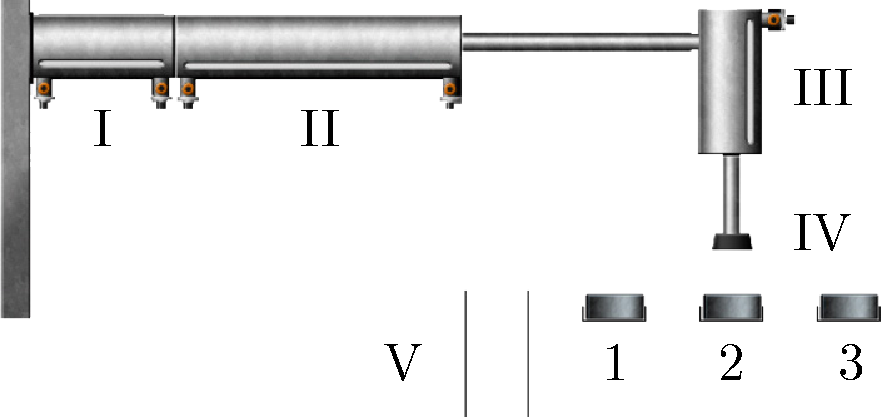
\includegraphics[width=8cm]{pnp-manipulator.pdf}
    \caption{Pick-and-Place манипулятор}
    \label{fig:pnp-manipulator}
\end{figure}

Pick-and-Place (PnP) манипулятор, изображенный на рисунке~\ref{fig:pnp-manipulator}, состоит из двух горизонтальных пневматических цилиндров~(I,~II), одного вертикального цилиндра~(III) и захватывающего устройства с вакуумной присоской~(IV) для подъема рабочий деталей.
Когда рабочая деталь оказывается во входном лотке (1,~2,~3), горизонтальные цилиндры располагают актюатор над деталью, вертикальный цилиндр опускает захватывающее устройство, который в свою очередь захватывает деталь, после чего вся система аналогичным образом приходит в движение для переноса захваченной детали в выходной лоток~(V).
Данная система управления реализована в соответствии со стандартом IEC~61499 с использованием функциональных блоков в среде моделирования nxtSTUDIO~\cite{nxtstudio}.
Логический контроллер, осуществляющий управление, выполнен в виде базового функционального блока, интерфейс которого включает в себя одно входное событие \texttt{REQ} (\textit{request}), одно выходное событие \texttt{CNF} (\textit{confirmation}), а также десять входных и семь выходных переменных.
Контроллер PnP\-/манипулятора оперирует следующими входными сигналами~$\SetInputVariables$, поступающими от объекта управления \--- среды исполнения:
\begin{itemize}[nosep]
    \item \texttt{c1Home}/\texttt{c1End} \--- горизонтальный цилиндр~I находится в крайнем левом/правом положении;
    \item \texttt{c2Home}/\texttt{c2End} \--- горизонтальный цилиндр~II находится в крайнем левом/правом положении;
    \item \texttt{vcHome}/\texttt{vcEnd} \--- вертикальный цилиндр~III находится в крайнем верхнем/нижнем положении;
    \item \texttt{pp1}/\texttt{pp2}/\texttt{pp3} \--- рабочая деталь находится на входном лотке~1/2/3;
    \item \texttt{vac} \--- вакуумная присоска включена.
\end{itemize}
В свою очередь контроллер PnP\-/манипулятора может посылать следующие сигналы~$\SetOutputVariables$ объекту управления:
\begin{itemize}[nosep]
    \item \texttt{c1Extend}/\texttt{c1Retract} \--- удлинить/\allowbreak{}втянуть цилиндр I;
    \item \texttt{c2Extend}/\texttt{c2Retract} \--- удлинить/\allowbreak{}втянуть цилиндр II;
    \item \texttt{vcExtend} \--- удлинить цилиндр III;
    \item \texttt{vacuum\_on}/\texttt{vacuum\_off} \--- включить/выключить ваккумную присоску.
\end{itemize}

% Данное исследование было нацелено на исследование практической применимости разработанных методов на примере синтеза описанного логического контроллера PnP\-/манипулятора.
% Процесс сбора сценариев исполнения (трассировок) для системы PnP\-/манипулятора описан в~\cite{fbCSP}.
% В данной работе были использованы наборы сценариев выполнения различных размеров: 1,~4, 10, 39 и 49 сценариев в каждом.


\subsection{Синтез минимальной конечно-автоматной модели по примерам поведения}%
\label{sub:exp-mono-pnp-scenarios-only}

Для исследования эффективности и практической применимости разработанных методов синтеза минимальных моделей по примерам поведения, производится сравнение с двухэтапным подходом из~\cite{chivilikhin-19}, где на первом этапе с помощью SAT-решателя строится базовая модели, удовлетворяющая заданым сценариям выполнения, а затем охранные условия полученной модели минимизируются с помощью CSP-решателя.
Стоит отметить, что превосходство данного двухэтапного метода над другими методами, например, EFSM-tools~\cite{efsm-tools}, уже было показано в~\cite{chivilikhin-19}, поэтому сравнение происходит только с двухэтапным методом, впоследствии называемым \enquote{Two-stage}.

Для синтеза минимальной конечно-автоматной модели контроллера PnP\-/манипулятора по заданным сценариям выполнения $\SetPositiveScenarios$ был применен алгоритм $\AlgoExtendedMinUB(\SetPositiveScenarios, w)$ с различными значениями параметра~$w$ \--- ширины плато для поиска локального минимума: $w = 0$ для случая, когда первое найденное решение считается финальным, $w = \infty$ для нахождения глобально-минимального решения, а также $w = 2$ для случая использования предложенной эвристики.
Результаты эксперимента представлены в Таблице~\ref{tab:results-monolith-pnp-extminub}, где
$\SetPositiveScenarios$ \--- набор сценариев выполнения,
$\card{\PositiveTree}$ \--- размер дерева сценариев;
\enquote{Время,~с} \--- время работы в секундах,
$\Nmin$ \--- минимальный суммарный размер охранных условий;
для метода Two\=/stage~\cite{chivilikhin-19}:
$\Cmin$ \--- минимальное число состояний,
$\Tmin$ \--- минимальное число переходов;
для метода $\AlgoExtendedMinUB$:
минимальное число состояний опущено, так как совпадает с $\Cmin$ для двухэтапного метода,
$P$ \--- максимальный размер каждого охранного условия,
$T$ \--- число переходов (не было минимизировано),
$w$ \--- критическая ширина плато для предложенной эвристики.
Результаты свидетельствуют о том, что разработанный метод $\AlgoExtendedMinUB$ способен генерировать более компактные конечные автоматны, чем двухэтапный метод, при этом значения эвристического параметра~${w = 2}$ достаточно для получения оптимального результата в терминах~$\Nmin$.

%% Table: Results for Extended-min-UB
\begin{table}[!htb]
    \centering
    \caption{Результаты синтеза минимальной конечно-автоматной модели логического контроллера PnP\-/манипулятора по примерам поведения с помощью двухэтапного метода Two-stage~\cite{chivilikhin-19} и алгоритма $\AlgoExtendedMinUB$}
    \label{tab:results-monolith-pnp-extminub}
    \subfile{tex/tab-mono-pnp-extminub-results}
\end{table}


\subsection{Синтез минимальный конечно-автоматных моделей по примерам поведения и LTL-спецификации}%
\label{sub:exp-mono-pnp-with-ltl}

%% Table: LTL properties
\begin{table}[p]
    \centering
    \caption{Темпоральные свойства для системы PnP\-/манипулятора}
    \label{tab:ltl-properties}
    \begin{adjustbox}{max width=\textwidth, max height=\maxheight{1}}
        \subfile{tex/tab-ltl-properties}
    \end{adjustbox}
\end{table}

Следующий эксперимент посвящен учету формальной спецификации с помощью применения индуктивного синтеза, основанного на контрпримерах.
Для использования LTL-свойств \textit{живости} (\textit{liveness}) верификация моделей с помощью NuSMV проводилась в замкнутом цикле~\cite{closed-loop} с заранее подготовленной формальной моделью объекта управления \--- PnP\-/манипулятора.
Эта модель определяет состояние объекта управления в зависимости от команд управления контроллера \--- синтезированной конечно-автоматной модели.
Набор использованых LTL-свойств представлен в таблице~\ref{tab:ltl-properties} и включает в себя как свойства безопасности \Prop{1}\==\Prop{6} (\enquote{система не окажется в нежелательном состояния}), так и свойства живости \Prop{7}\==\Prop{10} (\enquote{что-то полезное когда-нибудь произойдет}).
Свойства $\PropertiesConst$ \enquote{зафиксированы} \--- используются во всех экспериментах, в то время как использование свойств $\PropertiesVar$ варьируется.
Стоит отметить, что эти три свойства определяют тот факт, что если рабочая деталь (1\==3) размещается на входном лотке, то она когда-нибудь будет обработана.
Однако в оригинальной системе PnP\-/манипулятора~\cite{patil-pnp} выполняется \emph{только} свойство~\PropWP{1}, касающееся первой детали \--- если в первом входном лотке всегда присутствует рабочая деталь (при ее подъеме на ее месте в этот же момент появляется новая), то рабочие детали во втором и третьем входных лотках никогда не будут обработаны, что нарушает свойства живости \PropWP{2}~и~\PropWP{3}.
Поэтому каждое дополнительное (по отношению к~$\PropertiesConst$) свойство~$\PropertiesVar$ рассматривается отдельно от остальных, при этом предполагается, что рабочие детали появляются только на соответствующих входных лотках.
Для эксперимента с использованием дополнительного LTL-свойства~\PropWP{2} был использован специальный набор сценариев $\SetScenarios^{(1)\prime\prime}$, состоящий из одного сценария, описывающего обработку детали во втором входном лотке.
Аналогично, для свойства~$\PropWP{3}$ был использован специальный набор сценариев $\SetScenarios^{(1)\prime\prime\prime}$, состоящий из одного сценария, описывающего обработку детали в третьем входном лотке.

Проведенное экспериментальное сравнение включало в себя три метода: два разработанных метода $\AlgoCegis$ и $\AlgoCegisMin$, входящие в состав \smallcaps{fbSAT}, а также расширение метода \smallcaps{fbCSP} для учета LTL\-/спецификации, называемое впоследствии \mbox{\smallcaps{fbCSP+LTL}}~\cite{chivilikhin-18}.
Для обоих разработанных методов параметры $C^{*}$ и~$P^{*}$ были предварительно оценены с помощью алгоритма $\AlgoExtendedMinUB$ с параметром $w = 2$, время работы было учтено в суммарном времени работы алгоритма CEGIS\@.
% Для обоих разработанных методов использовалось значение параметра $w = 2$, эффективность которого была показана ранее (раздел~\ref{sub:exp-mono-pnp-scenarios-only}).
% Помимо времени работы методов и значения суммарного размера охранных условий $N$, также было учтено число итераций CEGIS\@.
Дополнительно, синтезированные модели были вручную протестированы в nxtSTUDIO~\cite{nxtstudio} \--- загружены в симуляционную среду и проверены на соответствие желаемому поведению.
Результаты данного экспериментального исследования представлены в таблице~\ref{tab:results-monolith-pnp-cegis}, где
\enquote{Дополнительное LTL-свойство} \--- одно из свойств $\PropertiesVar$, использованное в дополнение к свойствам $\PropertiesConst$,
$\SetPositiveScenarios$ \=== набор использованых позитивных сценариев выполнения $\SetPositiveScenarios$,
$N_{\text{init}}$ \--- начальный минимальный суммарный размер охранных условий (для автомата, полученного с помощью алгоритма $\AlgoExtendedMinUB(\SetPositiveScenarios, w)$),
\enquote{Время, с} \--- время работы в секундах,
$P$ \=== максимальный размер охранного условия,
$N$ \=== финальный суммарный размер охранных условий (при использовании алгоритма $\AlgoCegisMin$ это значения является минимальным),
\enquote{\#iter} \--- число итераций CEGIS\@.

%% Table: Results for CEGIS
\begin{table}[!htb]
    \centering
    \caption{Результаты применения подхода CEGIS к синтезу конечно-автоматной модели логического контроллера PnP\-/манипулятора по примерам поведения и LTL\-/спецификации}
    \label{tab:results-monolith-pnp-cegis}
    \subfile{tex/tab-mono-pnp-cegis-results}
\end{table}

Анализируя полученные результаты, можно заметить, что модели, найденные с помощью подхода CEGIS всегда имеют больший размер (в терминах суммарного размера охранных условий~$N$), нежели модели, построенные только по сценариям выполнения.
Это объясняется тем, что используемые сценарии выполнения не полностью покрывают рассмотренную LTL\-/спецификацию.
Поэтому алгоритм $\AlgoCegisMin$ всегда находит наименьшее решение и во всех случаях превосходит \mbox{\smallcaps{fbCSP+LTL}}~\cite{chivilikhin-18}, как по времени работы, так и по размеру моделей.
Наиболее интересным результатом является то, что $\AlgoCegisMin$ позволяет эффективно синтезировать модели по наборам сценариев $\SetScenarios^{(1)}$, $\SetScenarios^{(1)\prime\prime}$ и $\SetScenarios^{(1)\prime\prime\prime}$ \--- эти сценарии \enquote{не~покрывают} соответствующие свойства живости $\PropertiesVar$ в том смысле, что эти сценарии описывают процесс обработки только одной рабочей детали.
Существующий метод \smallcaps{fbCSP+LTL}~\cite{chivilikhin-18} не~справился в этих случаях, в то время как разработанный метод $\AlgoCegisMin$ с легкостью преуспел.
Также стоит отметить, что алгоритм $\AlgoCegis$ позволяет синтезировать модели быстрее, однако не обеспечивает минимальности охранных условий.


\section{Экспериментальное исследование: SYNTCOMP}%
\label{sec:experiments-monolith-syntcomp}

%% Weird boolvec notation from the original BoSy paper
\newcommand{\myboolvec}[1]{2^{#1}}

В этом разделе описывается применение разработанных методов к задаче синтеза системы переходов (\textit{transition system})~\cite{bosy,not-bosy} по входным данным с соревнования по реактивному синтезу SYNTCOMP~\cite{syntcomp}.
Один из треков соревнования SYNTCOMP \--- трек последовательного синтеза (\textit{sequential synthesis track}) \--- посвящен задаче синтеза системы переходов по заданной LTL\-/спецификации, также известной как задача LTL-синтеза.
Существует множество различных программных средств, осуществляющих LTL-синтез, среди которых можно выделить BoSy~\cite{bosy,not-bosy} и Strix~\cite{strix}.
Стоит отметить, что среди всех доступных программных средств только BoSy ограничивает размеры (число состояний) генерируемых систем переходов, однако BoSy не минимизирует размеры охранных условий, что значительно затрудняет анализ получаемых систем человеком.
Также стоит отметить, что на текущий момент разработанное в данной работе программное средство \smallcaps{fbSAT} неприменимо в явном виде к задаче LTL-синтеза, так как для \smallcaps{fbSAT} необходимым условием является наличие некоторого множества позитивных сценариев выполнения~$\SetPositiveScenarios$.
Несмотря на это, \smallcaps{fbSAT} может быть применен для \emph{минимизации} систем переходов, генерируемых BoSy.

Формально\footnote{%
    Здесь стоит отметить, что в данном разделе для описания системы переходов используется \emph{оригинальная} нотация из~\cite{not-bosy}.
    Эта нотация может конфликтовать с другими частями данной работы \--- следует считать, что все объявления в данном разделе действуют только здесь.
    Также стоит отметить, что в оригинальной нотации для обозначения \textit{множества всех наборов значений} пропозициональных переменных используется нотация $\myboolvec{X}$, где $X$ \--- множество пропозициональных переменных, однако более корректным обозначением было бы $\boolvec{X}$.
},
\textit{система переходов}~$\mathcal{T}$ это кортеж $\Tuple{ T, t_0, \Sigma = I \union O, \tau }$, где
$T$ \=== множество состояний,
$t_0 \in T$ \=== стартовое состояние,
$\Sigma$ \=== алфавит системы,
$I$ \=== множество пропозициональных переменных, управляемых окружением (\textit{входы}),
$O$ \=== множество пропозициональных переменных, управляемых системой (\textit{выходы}),
$\tau \colon T \times \myboolvec{I} \to \myboolvec{O} \times T$ \--- функция перехода, отображающая состояние~$t$ и входной набор $\bm{i} \in \myboolvec{I}$ в выходной набор $\bm{o} \in \myboolvec{O}$ и новое состояние~$t'$.
% $\Pair{t, \bm{i}} \mapsto \Pair{\bm{o}, t'}$
Можно заметить сходство систем переходов и конечно-автоматных моделей ECC базовых функциональных блоков.
Если система переходов обладает семантикой, схожей с семантикой автомата Мура (выходы в функции перехода зависят от состояния системы), то такая система может быть смоделирована в виде ECC, а значит и синтезирована с помощью \smallcaps{fbSAT}\@.

% \begin{equation}
%     \label{eq:moore-condition}
%     \forall t \in T
%     \ldotp
%     \forall \bm{i} \neq \bm{i}' \in \myboolvec{I}
%     \ldotp
%     \bigl[
%         \tau(t, \bm{i}) = \Pair{\bm{o}, \_\,}
%         \land
%         \tau(t, \bm{i}') = \Pair{\bm{o}', \_\,}
%     \bigr]
%     \implies
%     (\bm{o} = \bm{o}')
% \end{equation}

Наборы данных (\textit{инстансы}) на соревновании SYNTCOMP представляют собой JSON-файлы с описанием интерфейса системы и набора инвариантов \--- свойств на языке LTL, которые должны выполняться в каждый момент времени работы системы.
В листинге~\ref{lst:lilydemo19-json} приведен пример инстанса \texttt{lilydemo19}, описывающего систему с семантикой автомата Мили. Данная система оперирует входами $\Set{\texttt{ec}, \texttt{ets}}$ и выходами $\Set{\texttt{fl}, \texttt{hl}}$.
% В листинге~\ref{lst:full-arbiter-3-json} приведен пример инстанса \texttt{full\_arbiter\_3}, описывающего систему с семантикой автомата Мили. Данная система оперирует входами $\Set{r_0, r_1, r_2}$ и выходами $\Set{g_0, g_1, g_2}$.
Логика работы системы описывается с помощью LTL-свойств, указанных в поле \texttt{guarantees}, а~дополнительные глобальные ограничения (предположения) записаны в поле \texttt{assumptions}.

% TODO: fix listing
% \lstinputlisting[
%     float=!htb,
%     language=json,
%     % basicstyle=\small\ttfamily,
%     caption={Инстанс \texttt{lilydemo19.json}},
%     label={lst:lilydemo19-json}
% ]{data/lilydemo19.json}

%%% \lstinputlisting[
%%%     float=!htb,
%%%     language=json,
%%%     % basicstyle=\small\ttfamily,
%%%     caption={Инстанс \texttt{full\_arbiter\_3.json}},
%%%     label={lst:full-arbiter-3-json}
%%% ]{data/full_arbiter_3.json}

При выполнении данной работы был использован набор из 136 инстансов с соревнования SYNTCOMP~2018.
Для получения конечно-автоматных моделей в формате NuSMV по имеющимся LTL\-/спецификациям было использовано программное средство BoSy (input-symbolic, QBF-encoding, максимальное число состояний:~10, максимальное время работы:~1~час), в результате чего только только для 97 из~136 инстансов были получены результирующие модели.
В листинге~\ref{lst:lilydemo19-smv} приведена NuSMV модель для инстанса \texttt{lilydemo19}.
Все полученные модели были просимулированы с помощью NuSMV с целью получения случайных сценариев выполнения различных длин.
Для этого была использована команда `\verb/simulate -r -k <length>/' для симуляции (где `\verb/<length>/' \--- число шагов симуляции) и команда `\verb/show_traces -a -v/' для сохранения трассировок.
% TODO: restore this sentence after re-introducing the section {sec:scenarios}
% Полученные трассировки были сконвертированы в сценарии выполнения в соответствии с разделом~\ref{sec:scenarios}.

% TODO: fix listing
% \lstinputlisting[
%     float=!htb,
%     language=nusmv,
%     % basicstyle=\small\ttfamily,
%     caption={NuSMV модель для инстанса \texttt{lilydemo19}, сгенерированная BoSy},
%     label={lst:lilydemo19-smv}
% ]{data/lilydemo19.smv}

%%% \lstinputlisting[
%%%     float=!htb,
%%%     language=nusmv,
%%%     caption={NuSMV модель для инстанса \texttt{full\_arbiter\_3}, полученная с помощью BoSy},
%%%     label={lst:full-arbiter-3-smv}
%%% ]{data/full_arbiter_3.smv}

Полученные сценарии выполнения были использованы для синтеза конечно-автоматных моделей с помощью \smallcaps{fbSAT}.
На рисунке~\ref{fig:lilydemo19} представлена синтезированная модель для описанного выше инстанса \texttt{lilydemo19}.
Для синтеза было использовано пять сценариев длины~10 (\texttt{scenarios-k5-l10}), алгоритм $\AlgoExtendedMinUB(w = 0)$, время синтеза составило менее секунды.
Модель состоит из $C = 2$ состояний и $T = 4$ переходов, а охранные условия имеют суммарный размер $N = 6$.
Дополнительный этап верификации подтвердил соответствие синтезированной системы исходной LTL\-/спецификации, указанной во входном файле \texttt{lilydemo19.json}.
Как можно заметить, синтезированная модель полностью эквивалентна исходной NuSMV модели, поэтому необходимо рассмотрение более \enquote{сложного} инстанса.

%% Picture: lilydemo19 synthesized model
\begin{figure}[!htb]
    \centering
    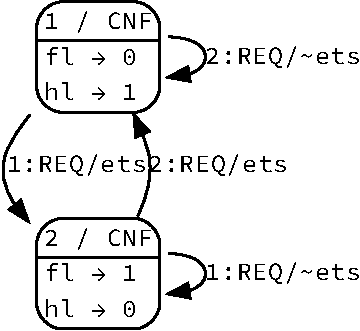
\includegraphics[max width=\textwidth]{lilydemo19.pdf}
    \caption{Конечно-автоматная модель для инстанса \texttt{lilydemo19}, синтезированная с помощью \smallcaps{fbSAT}}
    \label{fig:lilydemo19}
\end{figure}

Рассмотрим инстанс \texttt{full\_arbiter\_3} \--- данная система оперирует входами $\Set{r_0, r_1, r_2}$ и выходами $\Set{g_0, g_1, g_2}$.
Полученная с помощью BoSy система переходов $\mathcal{T}_{\text{original}}$ изображена на рисунке~\ref{fig:syntcomp-bosy} и состоит из $C = 8$ состояний и $T = 28$ переходов, а суммарный размер охранных условий $N = 147$.
На этом этапе можно предположить, что полученная модель не является минимальной, а значит, возможно применение \smallcaps{fbSAT} для синтеза минимальной модели, также соответствующей исходной LTL\-/спецификации \--- для этого был использован алгоритм $\AlgoCegisMin$.
Стоит заметить, что для более эффективного синтеза необходимо полное покрытие состояний сценариями выполнения. Поэтому было использовано 20~сценариев, каждый длины~20 (\texttt{scenarios-k20-l20}).

Стоит отметить, что формальное определение системы переходов, данное выше, не обязывает функцию переходов $\tau$ быть детерминированной, однако \smallcaps{fbSAT} всегда генерирует детерминированные модели.
Также стоит отметить, что формальное определение системы переходов не включает в себя функцию приоритета переходов, которая присутствует в определении ECC\@.
Для того, чтобы модели, синтезируемые \smallcaps{fbSAT}, соответствовали моделям, получаемым с помощью BoSy, в \smallcaps{fbSAT} было добавлено ограничение на \enquote{дизъюнктивные переходы}\footnote{Флаг \texttt{-{}-encode-disjunctive-transitions} в \smallcaps{fbSAT}} \--- в каждом состоянии $q \in \SetStates$ для каждого входа $u \in \SetTreeInputs$ выполняется не более одного перехода.
В результате была синтезирована модель $\Automaton_{\text{deterministic}}$, изображенная на рисунке~\ref{fig:syntcomp-fbsat-deterministic}, с тем же числом состояний и переходов, что и $\mathcal{T}_{\text{original}}$, однако с меньшим суммарным размером охранных условий: $N = 105$.

Если же не использовать введенное ограничение на \enquote{дизъюнктивные переходы}, а использовать \smallcaps{fbSAT} в оригинальном виде, то синтезируемые модели будут детерминированными ECC (из-за функции приоритета переходов), но недетерминированными системами переходов.
В таком случае результирующая модель $\Automaton_{\text{non-deterministic}}$, изображенная на рисунке~\ref{fig:syntcomp-fbsat}, обладает наименьшим суммарным размером охранных условий: $N = 52$.

Полученные результаты показывают, что предложенный подход к явному кодированию деревьев разбора булевых формул, соответствующих охранным условиям на переходах автомата, позволяет существенно сократить суммарный размер охранных условий в автомате.
Стоит также отметить, что данный подход применим не только \emph{после} LTL-синтеза \--- возможно расширить SAT-/QBF-сведение в BoSy предложенной кодировкой для охранных условий для их минимизации непосредственно \emph{в процессе} синтеза.


% \section{От монолитного синтеза к модульному}
% \label{sec:modular-intro}

% TODO: этот раздел действительно нужен, но нужно придумать какое-то содержание и краткий обзор того, что происходит в модульном синтезе

% Данная глава посвящена решению задачи синтеза модульных конечно-автоматных моделей с различными видами композиции модулей: (1)~параллельная (раздел~\ref{sec:modular-parallel-synthesis}), (2)~последовательная (раздел~\ref{sec:modular-consecutive-synthesis}) и (3)~произвольная (раздел~\ref{sec:modular-arbitrary-synthesis}).
% % TODO: distributed CEGIS section
% Раздел~\ref{sec:experiments-modular} содержит экспериментальное исследование, нацеленное на определение эффективности и применимости разработанных методов модульного синтеза.
% % В качестве модельной системы используется система Pick-and-Place манипулятора, уже рассмотренная ранее в разделе~\ref{sec:experiments-monolith-pnp}.
% % Несмотря на то, что оригинальная система фактически является монолитной, разработанные методы позволяют синтезировать распределенную модульную систему, обладающую схожим поведением.


% TODO: what is that?
% \subfile{tex/sec-composite-fb-model}

% \subfile{tex/sec-modular-parallel-synthesis}
\section{Метод синтеза модульных конечно-автоматных моделей с параллельной композицией модулей по примерам поведения}%
\label{sec:modular-parallel-synthesis}

В этом разделе рассматривается задача синтеза модульной конечно-автоматной модели с параллельной композицией модулей.
Аналогично монолитному синтезу (раздел~\ref{sec:automata-synthesis}), исходная задача сводится к задаче выполнимости SAT.
Полученное сведение состоит из двух компонент: (1)~определение переменных и (2)~определение ограничений.


\subsection{Сведение к SAT: переменные}%
\label{sub:modular-parallel-variables}

При параллельной композиции для описания каждого модуля~$m \in \Modules$ используются те же переменные, что и при монолитном синтезе \--- ко всем переменным добавляется верхний индекс~$(m)$.
Здесь и далее фраза \enquote{модуль~$m$} означает \enquote{модуль с номером~$m$}.
% TODO: Например, ... означает ... для модуля~$m$.
Дополнительно, объявляется переменная $\ModuleControllingOutputVariable_{z} \in \Modules$, кодирующая модуль, управляющий выходной переменной~$z \in Z$.
В данной постановке задачи рассматривается ситуация, когда каждый из модулей \enquote{управляет} своим собственным набором выходных переменных $\ModularSetOutputVariables \subset \SetOutputVariables$, причём эти наборы попарно не пересекаются.
Стоит отметить, что в общем случае эти наборы неизвестны заранее, а определяются динамически в ходе решения задачи SAT.
Возможна также ситуация, когда полное или частичное распределение переменных по модулям известно \--- в таком случае разработанный метод позволяет это учесть путём введения дополнительных ограничений на описанную переменную~$\ModuleControllingOutputVariable$.


\subsection{Сведение к SAT: ограничения}%
\label{sub:modular-parallel-constraints}

При модульном синтезе ограничения так же, как и при монолитном синтезе, делятся на две группы: (1)~ограничения, кодирующие структуру синтезируемого (модульного) автомата, (2)~ограничения, кодирующие соответствие поведения синтезируемого (модульного) автомата дереву сценариев.

Для кодирования структуры каждого модуля, входящего в состав модульного автомата, используются те же ограничения, что и при монолитном синтезе.
Дополнительно, вводятся следующие ограничения:
\begin{itemize}
    \item каждая выходная переменная $z \in \SetOutputVariables$ управляется ровно одним модулем:
    \[
        \ExactlyOne[m \in \Modules]{\ModuleControllingOutputVariable_{z} = m}
    \]

    \item каждый модуль $m \in \Modules$ управляет хотя бы одной выходной переменной:
    \[
        \AtLeastOne[z \in \SetOutputVariables]{\ModuleControllingOutputVariable_{z} = m}
    \]

    \item если выходная переменная $z \in \SetOutputVariables$ не управляется модулем~$m \in \Modules$, то алгоритмы во всех состояниях~$q \in \SetStates$ модуля~$m$ \enquote{ничего не делают} \--- переводят $\top$ в~$\top$ и $\bot$ в~$\bot$:
    \[
        (\ModuleControllingOutputVariable_{z} \neq m)
        \implies
        \bigland_{\mathclap{q \in \SetStates}}
        \Bigl[
            (\ModularStateAlgorithm_{q,z,\top} = \top)
            \land
            (\ModularStateAlgorithm_{q,z,\bot} = \bot)
        \Bigr]
    \]
\end{itemize}

В~свою очередь ограничения, кодирующие соответствие поведения синтезируемого модульного автомата дереву сценариев, отличаются от аналогичных при монолитном синтезе.
Для отображения пассивных вершин~$\SetTreeNodesPassive$ дерева сценариев используются те же ограничения, что и при монолитном синтезе.
А~при отображении активных вершин~$\SetTreeNodesActive$ дерева сценариев~$\PositiveTree$ на состояния~$\SetStates$ каждого модуля~$m \in \Modules$ необходимо дополнительно учитывать контролируемые этим модулем выходные переменные:
%
\begin{equation}
\label{eq:constraint-mapping}
\begin{split}
    \bigland_{m \in \Modules}
    \bigland_{v \in \SetTreeNodesActive}
    \bigland_{q \in Q}
    \biggl[
        (\ModularMapping_{v} = q)
        \iff
        % \implies
        \Bigl(
        (\ModularActualTransitionFunction_{q',e,u} = q)
        \land
        (\ModularStateOutputEvent_{q} = o)
        \land
        {}
        \Bigr.
    \biggr. \\
    \biggl.
        \Bigl.
        {}
        \land % from previous line
        \bigland_{\mathclap{z \in Z}}
        \bigl[
            (\ModuleControllingOutputVariable_{z} = m)
            \implies
            (\ModularStateAlgorithm_{q,z,\tov{p,z}} = \tov{v,z})
        \bigr]
        \Bigr)
    \biggr] ,
\end{split}
\end{equation}
где
$p = \tp{v}$,
$q' = \ModularMapping_{p}$,
$e = \tie{v}$,
$u = \tin{v}$,
$o = \toe{v}$.

% TODO: make modular output action?
Дополнительно, необходимо гарантировать корректность выходных событий модулей для соответствия дереву сценариев.
Для этого рассмотрим обработку модульным автоматом некоторого входного действия~$\InputAction$ из некоторой \textit{активной} вершины~$v$ дерева сценариев ($\toe{v} \neq \varepsilon$).
Каждый параллельный модуль $m \in \Modules$, входящий в состав модульного автомата, в ответ на входное действие генерирует выходное действие~$\OutputAction[(m)]$.
Возникает необходимость некоторым образом объединить эти выходные действия в одно~$\OutputAction$, которое будет являться финальной реакцией модульного автомата на исходное входное действие~$\InputAction$.
Фактически, необходимо использовать специальный функциональный блок, реализующий объединение событий и называемый \texttt{E\_MERGE} в IEC~61499.
Существует несколько способов такого объединения: (1)~синхронное \textit{rendezvous}, (2)~асинхронное \textit{rendezvous}, (3)~\textit{гибридное}.

Синхронное \textit{rendezvous} подразумевает ожидание завершения работы всех модулей, при этом корректной считается ситуация, когда выходные события всех модулей совпадают.
При формировании выходного действия~$\OutputAction$ используется общее выходное событие~$\OutputEvent$, а обновленные значения выходных переменных~$\OutputValues_{(m)}$ просто конкатенируются в~$\OutputValues$, так как множества~$\SetOutputVariables^{(m)}$ попарно не пересекаются.
Стоит отметить, что в этом случае ни один модуль не должен игнорировать входное действие \--- не должен генерировать пустое событие~$\OutputEvent = \varepsilon$.

\texttt{E\_MERGE} с асинхронным \textit{rendezvous} генерирует выходное действие равное входному, не ожидая завершения работы всех модулей
При этом модульный автомат, использующий такой тип объединения событий, в ответ на некоторое входное действие $\InputAction$ может реагировать несколькими выходными действиями.
Корректной считается следующая ситуация: каждый модуль генерируют либо выходное событие~$\OutputEvent$, либо пустое событие~$\varepsilon$; хотя бы один модуль генерирует непустое событие; объединение обновленных значений выходных переменных равно~$\OutputValues$.
Здесь~$\OutputAction$ \--- выходное действие, записанное в обрабатываемой активной вершине дерева сценариев.
Такая ситуация нарушает соответствие поведения модульного автомата дереву сценариев, однако может являться допустимой в реальном мире, так как последовательность выходных действий в ответ на одно входное все равно приводит систему к корректному состоянию с точки зрения значений выходных переменных.

Гибридный способ объединения событий является совокупностью синхронного и асинхронного \textit{rendezvous}.
Гибридный \texttt{E\_MERGE} генерирует ровно одно выходное событие (\enquote{асинхронное} поведение), при этом непустых входных событий может быть несколько, и все они учитываются для генерации совместного события.
Это достигается тем, что гибридный блок ожидает завершения работы всех модулей (\enquote{синхронное} поведение) лишь некоторое ограниченное время.
При этом считается, что все неответившие модули игнорировали входное действие, а значит, продуцировали пустое выходное событие~$\varepsilon$.
Корректной считается ситуация, когда каждый модуль генерируют либо выходное событие~$\OutputEvent$, либо пустое событие~$\varepsilon$, а объединение обновленных значений выходных переменных равно~$\OutputValues$, где $\OutputAction$ \=== выходное действие, записанное в обрабатываемой активной вершине дерева сценариев.

В приведенном выше ограничении (\ref{eq:constraint-mapping}), кодирующем отображение активных вершин дерева на состояния модулей, используется синхронный вариант объединения выходных событий.
% TODO: Потому что...


\subsection{Алгоритмы \AlgoModularParallelBasic\ и \AlgoModularParallelExtended}%
\label{sub:algorithm-modular-parallel-basic-and-extended}

Обозначим $\AlgoModularParallelBasicFull(\SetPositiveScenarios, M, C, T)$ алгоритм, реализующий синтез модели, удовлетворяющей заданным сценариям выполнения $\SetPositiveScenarios$ и состоящей из $M$ \textit{параллельно} соединенных модулей, каждый из которых состоит из $C$ состояний (суммарное число состояний равно~${M \cdot C}$), а суммарное число переходов во всех модулях не больше~$T$.
Также введём обозначение для случая, когда число переходов в автомате остается неограниченным:
\[
    \AlgoModularParallelBasic(\SetPositiveScenarios, M, C) = \AlgoModularParallelBasicFull(\SetPositiveScenarios, M, C, {T = \infty})
\]

Отметим, что модификации сведения для синтеза расширенных моделей не отличаются от описанных в главе~\ref{ch:automata-synthesis} \--- структура охранных условий кодируется независимо от количества модулей и их композиции.
Поэтому здесь и далее алгоритмы, реализующие синтез расширенных моделей, будут объявляться без пояснений:
% $\AlgoModularParallelExtendedFull(\SetPositiveScenarios, M, C, P, N)$, а также отдельное обозначение:
\begin{align*}
    & \AlgoModularParallelExtended(\SetPositiveScenarios, M, C, P) = \\
    & = \AlgoModularParallelExtendedFull(\SetPositiveScenarios, M, C, P, {N = \infty})
\end{align*}


% \subfile{tex/sec-modular-consecutive-synthesis}
\section{Метод синтеза конечно-автоматной модели модульного логического контроллера с последовательной композицией модулей по примерам поведения}%
\label{sec:modular-consecutive-synthesis}

Последовательная композиция модулей значительно отличается от параллельной, так как модули в таком случае перестают быть независимыми \--- каждый следующий модуль зависит от предыдущего.
В данной работе рассматривалась постановка задачи синтеза модульного контроллера со следующими особенностями и допущениями: (1)~каждый модуль зависит от всех входных переменных \textit{внешнего} (модульного) автомата, (2)~значения выходных переменных каждого модуля зависят от предыдущих значений выходных переменных предыдущего модуля (для первого модуля \enquote{предыдущим} считается он сам), (3)~входное событие обрабатывается (происходит генерация ответного выходного события) только последним модулем, до которого оно неизменно передается от модуля к модулю.
% TODO: картинка


\subsection{Сведение к SAT: переменные}%
\label{sub:modular-consecutive-variables}

Аналогично параллельной композиции, структура каждого модуля кодируется так же, как и при монолитном синтезе, с учетом допущения о том, что только последний модуль реагирует на входные события, а все предыдущие модули просто неизменно передают полученное входное событие далее \--- это достигается тем, что множества выходных событий каждого модуля приравниваются множеству входных событий:
\[
    \forall m \in [1..(M-1)] : {\ModularSetOutputEvents = \SetInputEvents} %.
\]
Дополнительно, объявляется переменная~$\ModularComputedValue_{v,z} \in \Bool$, кодирующая \enquote{вычисленное} значение выходной переменной~$z \in \SetOutputVariables$ при отображении каждой вершины~$v \in \SetTreeNodes$ дерева сценариев \--- значение в каждый момент времени после обработки соответствующей вершины дерева.


\subsection{Сведение к SAT: ограничения}%
\label{sub:modular-consecutive-constraints}

Для определения переменной $\ModularComputedValue$ объявляются следующие ограничения.
Изначально, в момент времени после \enquote{обработки} фиктивного корня~$\TreeRoot$ дерева сценариев, вычисленные значения всех выходных переменных~$z \in \SetOutputVariables$ во всех модулях~$m \in \Modules$ равны \texttt{False}:
\[
    \bigland_{m \in \Modules}
    \bigland_{z \in \SetOutputVariables}
    (\ModularComputedValue_{\TreeRoot,z} = \bot) %.
\]
В следующие моменты времени, при обработке вершин $v \in \SetTreeNodes \setminus \{ \TreeRoot \}$, вычисляемые значения выходных переменных определяются в соответствии с работой алгоритмов в состояниях, в которых в эти моменты времени находятся модули \--- в тех состояниях, в которые отображаются рассматриваемые вершины дерева сценариев:~$\ModularMapping_{v}$.
Для первого модуля:
\[
    \bigland_{v \in \SetTreeNodes \setminus \{ \TreeRoot \}}
    \bigland_{z \in \SetOutputVariables}
    \Bigl[
        \ModularComputedValue_{v,z}
        \iff
        \ModularStateAlgorithm_{\ModularMapping_{v},z,\tov{\tp{v},z}}
    \Bigr] %.
\]
Для последующих модулей:
\[
    \bigland_{m \in [2 \twodots M]}
    \bigland_{v \in \SetTreeNodes \setminus \Set{\TreeRoot}}
    \bigland_{z \in \SetOutputVariables}
    \Bigl[
        \ModularComputedValue_{v,z}
        \iff
        \ModularStateAlgorithm_{\ModularMapping_{v},z,\ModularComputedValue[m-1]_{v,z}}
    \Bigr] %.
\]

При отображении активных вершин дерева необходимо учесть, что все модули, кроме последнего, передают входное событие следующему модулю. Стоит отметить, что при этом реакция модулей на входные события не изменяется \--- входные события так же играют свою роль в охранных условиях на переходах автомата.
Также необходимо учесть, что значения выходных переменных ограничиваются для соответствия дереву сценариев только для последнего модуля \--- все предыдущие модули могут производить произвольные операции над выходными переменными в рамках существующего сведения.
\begin{gather*}
    \bigland_{v \in \SetTreeNodesActive}
    \bigland_{m \in [1..(M-1)]}
    \bigland_{q \in Q}
    \Bigl[
        (\ModularMapping_{v} = q)
        \implies
        \bigl(
            (\ModularActualTransitionFunction_{q',e,u} = q)
            \land
            % Note: "outputevent = e", THIS IS NOT A TYPO
            (\ModularStateOutputEvent_{q} = e)
        \bigr)
    \Bigr] , \\
    \bigland_{v \in \SetTreeNodesActive}
    \bigland_{q \in Q}
    \Bigl[
        (\ModularMapping[M]_{v} = q)
        \implies
        \bigl(
            (\ModularActualTransitionFunction[M]_{q',e,u} = q)
            \land
            (\ModularStateOutputEvent[M]_{q} = o)
            \land
            \bigland_{\mathclap{z \in \SetOutputVariables}}
            (\ModularComputedValue[M]_{v,z} = \tov{v,z})
        \bigr)
    \Bigr] ,
\end{gather*}
где
$p = \tp{v}$,
$q' = \ModularMapping_{p}$,
$e = \tie{v}$,
$u = \tin{v}$.

При отображения пассивных вершин достаточно закодировать тот факт, что все модули игнорируют входное воздействие \--- автоматы не изменяют своего состояния:
\[
    \bigland_{v \in \SetTreeNodesPassive}
    \bigland_{m \in \Modules}
    % TODO: check whether "= q_0" is correct, originally was "= 0"
    (\ModularActualTransitionFunction_{q',e,u} = q_0) ,
\]
где
$p = \tp{v}$,
$q' = \ModularMapping_{p}$,
$e = \tie{v}$,
$u = \tin{v}$.


\subsection{Алгоритмы \AlgoModularConsecutiveBasic\ и \AlgoModularConsecutiveExtended}%
\label{sub:algorithm-modular-consecutive-basic-and-extended}

Аналогично разделу~\ref{sub:algorithm-modular-parallel-basic-and-extended}, обозначим $\AlgoModularConsecutiveBasicFull(\SetPositiveScenarios, M, C, T)$ алгоритм, реализующий синтез модульной модели с \textit{последовательной} композицией модулей.
Также введём обозначение для случая, когда число переходов в автомате остается неограниченным:
\begin{align*}
    & \AlgoModularConsecutiveBasic(\SetPositiveScenarios, M, C) = \\
    & = \AlgoModularConsecutiveBasicFull(\SetPositiveScenarios, M, C, {T = \infty}) %.
\end{align*}
В соответствии с разделом~\ref{sub:algorithm-modular-parallel-basic-and-extended}, алгоритм для синтеза расширенных моделей объявляется без пояснений:
\begin{align*}
    & \AlgoModularConsecutiveExtended(\SetPositiveScenarios, M, C, P) = \\
    & = \AlgoModularConsecutiveExtendedFull(\SetPositiveScenarios, M, C, P, {N = \infty}) %.
\end{align*}


\section{Метод синтеза модульных конечно-автоматных моделей с произвольной композицией модулей по примерам поведения}%
\label{sec:modular-arbitrary-synthesis}

Наиболее общей формулировкой задачи синтеза конечно-автоматных моделей логических контроллеров является модульный синтез с произвольной композицией модулей.
Каждый модуль рассматривается как черный ящик с набором входных и выходных контактов для входных/выходных событий/переменных. Содержимое черного ящика \--- монолитный контроллер, структура которого кодируется так же, как при монолитном синтезе.
Совокупность модулей является внутренним содержимым модульного контроллера, так же обладающего входными и выходными \textit{контактами}.
Контакты соединяются \textit{связями}, что обеспечивает взаимодействие модулей друг с другом.
При такой постановке задачи, разрабатываемый метод обладает максимальными возможностями для синтеза комплексных модульных структур, и является свободным от ограничений, присущих рассмотренным ранее параллельной и последовательной композициям.
Стоит отметить, что для корректных вычислений выходных событий и значений выходных переменных необходимо знать порядок вычисления модулей, что возможно только если граф связей модулей является ацикличным.
Данное ограничение не уменьшает вычислительной способности модульного контроллера, поэтому в данной работе предполагается, что граф связей модулей является ацикличным, а также то, что модули упорядочены в порядке их номеров: от~1 до~$M$.

% \begin{figure}
%     % \includegraphics[max width=0.9\textwidth]{img/modular.png}
%     \includegraphics[max width=0.9\textwidth]{img/modular_full.png}
%     \caption{Пример модульного автомата с произвольной композицией}%
%     % \label{fig:my_label}
% \end{figure}


\subsection{Сведение к SAT: переменные}%
\label{sub:modular-arbitrary-variables}

Рассмотрим подробнее, как устроено сведение для модульного синтеза с произвольной композицией.
Обозначим $\ModularSetInboundVarPins = \{ {(m-1) \cdot \card{\SetInputVariables} + 1}, \dots, {m \cdot \card{\SetInputVariables}} \}$ множество входных контактов для переменных, считая, что контакты нумеруются натуральными числами, начиная с единицы, а нумерация является сквозной среди всех модулей~$m \in \Modules$ для всех контактов одного типа.
Аналогично, обозначим~$\ModularSetOutboundVarPins$ множество выходных контактов для переменных, а также обозначим множества входных и выходных контактов для событий $\ModularSetInboundEventPins$ и~$\ModularSetOutboundEventPins$.
Дополнительно, обозначим множества контактов для внешнего (модульного) автомата следующим образом: $\SetExternalInboundVarPins$, $\SetExternalOutboundVarPins$, $\SetExternalInboundEventPins$,~$\SetExternalOutboundEventPins$.
Отметим, что, например, множество~$\SetExternalInboundVarPins$ внешних входных контактов для переменных соответствует выходным переменным~$\SetOutputVariables$, так как эти контакты являются входами для входящих в них связей из выходных контактов.
При этом нумерация внешних контактов продолжает нумерацию модульных того же типа, например, $\SetExternalInboundVarPins = \{ {M \cdot \card{\SetInputVariables} + 1}, \dots, {M \cdot \card{\SetInputVariables} + \card{\SetOutputVariables}} \}$.
Для упрощения используемой нотации обозначим множества \emph{всех} входных/выходных контактов для переменных/событий $\SetInboundVarPins$, $\SetOutboundVarPins$, $\SetInboundEventPins$,~$\SetOutboundEventPins$, где, например:
\[
    \SetInboundVarPins = \SetExternalInboundVarPins \union \bigunion_{\mathclap{m \in \Modules}} \ModularSetInboundVarPins %.
\]

Следующий шаг \--- определение графа соединений контактов модулей.
Введём переменные $\VarPinParent_{p} \in \SetOutboundVarPins$ и~$\EventPinParent_{p} \in \SetOutboundEventPins$, обозначающие родителя входного контакта~$p$ для переменных/событий.
Можно заметить, что родителем входного контакта может быть только выходной контакт.
Если контакт является родителем другого, то они соединены \textit{связью}, и обновление значения родителя приводит к обновлению значения ребенка.
Пользуясь допущением об ацикличности графа соединений модулей, определим, что родителем входного контакта~$p$ может быть выходной контакт из модуля с меньшим номером, либо внешний выходной контакт, например, для некоторого контакта~$p \in \SetInboundVarPins$ из модуля~$m$:
\[
    \VarPinParent_{p} \in \SetExternalOutboundVarPins \union \bigunion_{\mathclap{m' < m}} \ModularSetOutboundVarPins[m'] %.
\]

Для каждого контакта необходимо кодировать его вычисленное значение в каждый момент времени в процессе отображения вершин дерева сценариев на состояния модулей.
Для этого вводятся переменные $\InboundVarPinComputedValue_{v,p'}$ и~$\OutboundVarPinComputedValue_{v,p''}$, кодирующие значения входных и выходных контактов ${p' \in \SetInboundVarPins}$ и ${p'' \in \SetOutboundVarPins}$ в момент времени после обработки вершины~$v$ дерева сценариев.

Важно отметить, что в отличие от рассмотренных ранее методов, при произвольной композиции каждый модуль может получать на вход произвольные наборы значений входных переменных.
Всего существует $2^{\card{\SetInputVariables}}$ таких наборов, и каждый из них должен быть корректно обработан каждым модулем.
Поэтому при кодировании структуры автомата необходимо учитывать множество всех возможных различных входов $\SetAllInputs = \boolvec{\SetInputVariables} = \{ \Vector{0 \dots 0}, \dots, \Vector{1 \dots 1} \}$, а не только множество входов $\SetTreeInputs \subseteq \SetAllInputs$, встречающихся в дереве сценариев.
Введём переменную~$\ModularInputIndex_{v} \in \SetAllInputs$, обозначающую вход в момент времени после обработки вершины~$v$ дерева сценариев.
Заметим, что вычисленные значения~$\InboundVarPinComputedValue_{v,p}$ входных контактов являются битами в бинарной записи номера входа~$u \in \SetAllInputs$, учитывая, что входы нумеруются с нуля.
Для взаимосвязи этих двух переменных была использована техника кодирования целочисленных SAT переменных OneHot+Binary~\cite{sat-encodings}: числовое значение переменной~$\ModularInputIndex_{v}$ соответствует номеру входа~$u \in \SetAllInputs$, а биты соответствующего двоичного числа \--- значениям переменной~$\InboundVarPinComputedValue_{v,p}$.


\subsection{Сведение к SAT: ограничения}%
\label{sub:modular-arbitrary-constraints}

Для определения переменных $\InboundVarPinComputedValue_{v,p}$ и $\OutboundVarPinComputedValue_{v,p}$ объявляются следующие ограничения:
\begin{enumerate}
% DC: СТОИТ НАПИСАТЬ СЛОВАМИ, КАКАЯ ИМЕННО
\item Взаимосвязь родителя контакта с его потомком:
\[
    \bigland_{v \in \SetTreeNodes}
    \bigland_{p \in \SetInboundVarPins}
    \Bigl[
        \OutboundVarPinComputedValue_{v,p}
        \iff
        \InboundVarPinComputedValue_{v,\VarPinParent_{p}}
    \Bigr]
\]

\item Начальные значения всех выходных контактов равны \texttt{False}:
\[
    \bigland_{p \in \SetOutboundVarPins}
    (\OutboundVarPinComputedValue_{1,p} = \bot)
\]

\item Значения входных переменных, записанные в вершинах дерева (кроме корня):
\[
    \bigland_{v \in \SetTreeNodes \setminus \Set{\TreeRoot}}
    \bigland_{p \in \SetExternalOutboundVarPins}
    (\OutboundVarPinComputedValue_{v,p} = \tiv{v,\funcname{pinToInputVar}(p)}) ,
\]
где $\funcname{pinToInputVar} \colon \SetExternalOutboundVarPins \to \SetInputVariables$ \--- функция, возвращающая входную переменную $x \in \SetInputVariables$, соответствующую внешнему выходному контакту $p \in \SetExternalOutboundVarPins$.

\item Значения входных контактов, у которых нет родителей, принимаются равными \texttt{False}:
\[
    \bigland_{p \in \SetInboundVarPins}
    \Bigl[
        (\VarPinParent_{p} = 0)
        \implies
        \bigland_{v \in \SetTreeNodes}
        (\InboundVarPinComputedValue_{v,p} = \bot)
    \Bigr] %.
\]
\end{enumerate}

При отображении активных вершин дерева сценариев на состояния модулей необходимо учитывать новую переменную~$\ModularInputIndex$:
\[
    \bigland_{m \in \Modules}
    \bigland_{v \in \SetTreeNodes}
    \Bigl[
        (\ModularMapping_{v} = q)
        \implies
        (\ModularActualTransitionFunction_{q',u} = q)
    \Bigr] ,
\]
где $p = \tp{v}$, $q' = \ModularMapping_{p}$, $u = \ModularInputIndex_{v}$.

Вычисляемые значения выходных контактов модулей зависят от своих предыдущих значений и определяются с помощью алгоритмов в состояниях модулей:
\[
    \bigland_{m \in \Modules}
    \bigland_{v \in \SetTreeNodes}
    \bigland_{p \in \SetOutboundVarPins}
    \bigland_{z \in \SetOutputVariables}
    \Bigl[
        \OutboundVarPinComputedValue_{v,p}
        \iff
        \fun{ITE}(\OutboundVarPinComputedValue_{v',p}, \ModularStateAlgorithm_{q,z,\top}, \ModularStateAlgorithm_{q,z,\bot})
    \Bigr] ,
\]
где $v' = \tp{v}$, $q = \ModularMapping_{v}$.
Также необходимо ограничить значения внешних входных контактов (напомним, что эти контакты соответствуют выходным переменным внешнего модульного автомата) в соответствии со значениями в дереве сценариев:
\[
    \bigland_{v \in \SetTreeNodes}
    \bigland_{p \in \SetExternalInboundVarPins}
    \Bigl[
        \InboundVarPinComputedValue_{v,p} = \tov{v, \funcname{pinToOutputVar}(p)}
    \Bigr] ,
\]
где $\funcname{pinToOutputVar}(p) \colon \SetExternalInboundVarPins \to \SetOutputVariables$ \--- функция, возвращающая выходную переменную~$z \in \SetOutputVariables$, соответствующую внешнему входному контакту~$p \in \SetExternalInboundVarPins$.

% DC: Кстати, в общем случае это, вероятно, не так. Некоторые модули могут что-то делать. Нам достаточно потребовать, что на выход не передается события, а переменные не изменяют своих значений. Можно также упомянуть про это и указать, что мы сейчас используем такое упрощение.
При отображении пассивных вершин достаточно закодировать тот факт, что все модули игнорируют входное действие, записанное в вершине дерева сценариев. При этом необходимо учесть нововведенную переменную~$\ModularInputIndex$:
\[
    \bigland_{m \in \Modules}
    \bigland_{v \in \SetTreeNodesPassive}
    \Bigl[
        (\ModularMapping_{v} = \ModularMapping_{\tp{v}})
        \land
        (\ModularActualTransitionFunction_{q',u} = 0)
    \Bigr] ,
\]
где $q' = \ModularMapping_{\tp{v}}$, $u = \ModularInputIndex_{v}$.
Также, значения выходных контактов не изменяются, так как модули не генерируют выходных событий:
\[
    \bigland_{v \in \SetTreeNodesPassive}
    \bigland_{p \in \SetOutboundVarPins}
    (\OutboundVarPinComputedValue_{v,p} = \OutboundVarPinComputedValue_{\tp{v},p})
    %.
\]


\subsection{Алгоритмы \AlgoModularArbitraryBasic\ и \AlgoModularArbitraryExtended}%
\label{sub:algorithm-modular-arbitrary-basic-and-extended}

Аналогично разделу~\ref{sub:algorithm-modular-parallel-basic-and-extended}, обозначим $\AlgoModularArbitraryBasicFull(\SetPositiveScenarios, M, C, T)$ алгоритм, реализующий синтез модульной модели с \textit{произвольной} композицией модулей.
Также введём обозначение для случая, когда число переходов в автомате остается неограниченным:
\begin{align*}
    & \AlgoModularArbitraryBasic(\SetPositiveScenarios, M, C) = \\
    & = \AlgoModularArbitraryBasicFull(\SetPositiveScenarios, M, C, {T = \infty}) %.
\end{align*}
В соответствии с разделом~\ref{sub:algorithm-modular-parallel-basic-and-extended}, алгоритм для синтеза расширенных моделей объявляется без пояснений:
\begin{align*}
    & \AlgoModularArbitraryExtended(\SetPositiveScenarios, M, C, P) = \\
    & = \AlgoModularArbitraryExtendedFull(\SetPositiveScenarios, M, C, P, {N = \infty})
\end{align*}


\section{Синтез минимальных модульных конечно-автоматных моделей}%
\label{sec:synth-minimal-modular-models}

% В этом разделе рассматривается итеративный подход к синтезу минимальных модульных моделей, аналогичный рассмотренному в разделе~\ref{sec:synth-minimal-models}.

Для синтеза \emph{минимальных} модульных моделей в данной работе используется тот же итеративный подход, что и при монолитном синтезе (раздел~\ref{sec:synth-minimal-models}).

Алгоритм $\AlgoModularParallelBasicMin(\SetPositiveScenarios, M)$ позволяет синтезировать базовую конечно-автоматную модель композитного функционального блока с параллельной композицией заданного числа модулей~$M$ с минимальным числом состояний и переходов.
При минимизации предполагается, что все модули имеют одинаковое число состояний, а число переходов считается суммарно во всех модулях.
Возможно также рассмотрение такой постановки задачи, когда размеры каждого модуля заданы явно (или в виде некоторых интервальных оценок), однако в общем случае эти значения абсолютно неизвестны заранее.
В результате минимальная модульная модель содержит~${M \cdot \Cmin}$ состояний (по~$\Cmin$ в каждом модуле) и $\Tmin = \Tmin^{(1)} + \dotsb + \Tmin^{(M)}$ переходов.
Здесь стоит отметить, что используемая нотация~$\Tmin^{(m)}$ обозначает \textit{возможно неминимальное} число переходов в модуле~${m \in \Modules}$, входящего в состав \textit{минимальной} модульной модели с \textit{минимальным} суммарным числом переходов~$\Tmin$.

Аналогично, алгоритм $\AlgoModularParallelExtendedMin(\SetPositiveScenarios, M, P)$ позволяет синтезировать расширенную модульную модель с параллельной композицией $M$~модулей с минимальным числом состояний~${M \cdot \Cmin}$, минимальным суммарным размером охранных условий~$\Nmin$ и максимальным размером каждого охранного условия~$P$.

Аналогичным образом определяются алгоритмы для синтеза базовых и расширенных модульных моделей с последовательной и произвольной композиций модулей:
\begin{itemize}[nosep]
    \item $\AlgoModularConsecutiveBasicMin(\SetPositiveScenarios, M)$: базовая/последовательная;
    \item $\AlgoModularConsecutiveExtendedMin(\SetPositiveScenarios, M, P)$: расширенная/последовательная;
    \item $\AlgoModularArbitraryBasicMin(\SetPositiveScenarios, M)$: базовая/произвольная;
    \item $\AlgoModularArbitraryExtendedMin(\SetPositiveScenarios, M, P)$: расширенная/произвольная.
\end{itemize}



% \section{From Monolithic to Distributed Synthesis}%
% \label{sec:distributed}

% This paper proposes an extension of the \com{fbSAT} approach~\cite{fbSAT-arXiv} described in the previous section.
% The proposed extension allows for synthesis of distributed controllers, and is based on two ideas.
% The first one is to declare a reduction for monolithic case for each module independently.
% This is described in \cref{sec:distributed:modular}.
% The second idea has to do with the adaptation of CEGIS developed in~\cite{fbSAT-arXiv} to make it applicable for distributed synthesis, and is the main idea of the paper.
% % The most important difference from the monolithic case arises in the implementation of CEGIS\@.
% The difficulty of using CEGIS for distributed synthesis is that since the specification is written for the system as a whole, negative scenarios derived from counterexamples are also written for the system as a whole.
% % \commentDC{The previous sentence is imperfect, too. We should directly emphasize that since the specification is written for the distributed system as a whole, counterexamples generated by the model checker are also in terms of the system as a whole. And the question is how to deal with these counterexamples.}
% \Cref{sec:distributed:construction} describes the structure of these scenarios.
% The difficulty is that it is not known in advance, which modules behave incorrectly in some particular negative scenario, and thus we do not know, in which module do we need to prohibit the negative scenario.

% The na\"ive approach would be to prohibit each negative scenario for all modules, but it would be incorrect to do so: a behavior that is incorrect for one of the modules may be completely normal for another one.
% Thus, this na\"ive approach would lead to unsatisfiability of corresponding Boolean formulas, and the sought distributed controller would not be synthesized.

% The key idea to cope with this difficulty is to make sure that each negative scenario is prohibited for at least one module.
% This is described in \cref{sec:distributed:mapping}.
% Finally, in \cref{sec:distributed:minimal} we discuss the algorithm for minimization of inferred automata in terms of their parameters, \eg number of states and total size of guard conditions.


\section{От монолитного к распределённому синтезу}
\label{sec:distributed}

% TODO: REFORMULATE
% В данной работе предлагается расширение подхода, описанного в разделе .
Предлагаемое расширение позволяет осуществлять синтез моделей распределённых систем и основывается на двух идеях.
Первая идея заключается в том, чтобы для каждого модуля в распределённой системе независимо кодировать задачу монолитного синтеза в SAT.
Это описано в разделе~\ref{sec:distributed:modular}.
Вторая идея связана с адаптацией подхода CEGIS, описанного и использованного в разделе~\ref{sec:cegis}, с целью сделать его применимым для распределённого синтеза.

Сложность использования CEGIS для распределённого синтеза заключается в том, что поскольку спецификация написана для системы \emph{в целом}, негативные сценарии, полученные из контрпримеров, также описывают (негативное) поведение системы в целом.
Раздел~\ref{sec:distributed:construction} описывает структуру этих сценариев.
Проблема заключается в том, что заранее неизвестно, какие именно модули ведут себя неправильно в конкретном негативном сценарии, и, следовательно, неизвестно, в каком модуле необходимо запретить данный негативный сценарий.

Наивный подход заключался бы в том, чтобы запретить каждый негативный сценарий для всех модулей, но это было бы некорректно: поведение, которое является неправильным для одного из модулей, может быть совершенно нормальным для другого.
Таким образом, этот наивный подход привёл бы к невыполнимости соответствующих булевых формул, и искомая распределённая система не была бы синтезирована.

Ключевая идея для преодоления этой проблемы заключается в том, чтобы убедиться, что каждый негативный сценарий запрещён хотя бы для одного модуля.
Это описано в разделе~\ref{sec:distributed:mapping}.
Наконец, в разделе~\ref{sec:distributed:minimal} обсуждается алгоритм синтеза минимальных автоматов с точки зрения их параметров, например, количества состояний и суммарного размера охранных условий.


% \subsection{Reduction for distributed synthesis from positive scenarios}%
% \label{sec:distributed:modular}

% We declare the reduction described in \cref{sec:monolithic} for each module independently, adding the module index to every variable.
% Thus, respective constraints remain the same, but are now quantified over all modules.
% For instance, variable \(\ModularTransitionDestination_{q,k} \in \SetStatesAux\) denotes the destination state of the~$k$-th transition from state~$q$ in the automaton for the~$m$-th module, and variable \(\ModularTransitionInputEvent_{q,k} \in \SetInputEvents \union \{\varepsilon\}\) denotes the input event associated with that transition.
% With the constraint \(
%     (\ModularTransitionDestination_{q,k} = q_0) \iff (\ModularTransitionInputEvent_{q,k} = \varepsilon)
% \) we enforce that only transitions to $q_0$ are marked with the $\varepsilon$ input event.
% We also add module indices to the reduction parameters. For example, $\ModularC$ denotes the number of states in $\ModularAutomaton$ \--- the automaton for the~$m$-th module.
% All other parts of the encoding from \cref{sec:monolithic} are extended in a similar way, except for the negative mapping, which we discuss below.

% The difference with positive scenarios is that now we have a set of positive scenario trees $\Set{\ModularPositiveTree}_{m \in \Modules}$, one for each module of the distributed controller.
% % , where $\ModularPositiveTree$ is a positive scenario tree for the $m$-th module.
% Variable $\ModularMapping_{v}$ denotes a state in which the automaton for the $m$-th module finishes processing a sequence of inputs formed by following the positive tree from the root till the node~$v$ (since the tree is deterministic, for each node $v$ there is only one path from the root).
% This variable represents a mapping $\ModularMapping_{} : \ModularSetTreeNodes \to \ModularSetStates$ between the nodes of $\ModularPositiveTree$ and the states of an automaton $\ModularAutomaton$, and the constraints on this mapping are the same to those described in \cref{sec:monolithic:positive}.


\subsection{Сведение к SAT для распределённого синтеза по примерам поведения}
\label{sec:distributed:modular}

В данном подразделе представлено сведение к SAT, основа которого уже была описана в разделе~\ref{sec:monolithic}.
Для каждого модуля независимо объявляется описанный набор переменных и ограничений \--- ко всем переменным в сведении добавляется индекс модуля.
Таким образом, соответствующие ограничения остаются теми же, но теперь они также квантифицированы по всем модулям.
Например, переменная $\ModularTransitionDestination_{q,k} \in \SetStatesAux$ обозначает конечное состояние $k$-го перехода из состояния~$q$ в автомате для $m$-го модуля, а переменная $\ModularTransitionInputEvent_{q,k} \in \SetInputEvents \union \{\varepsilon\}$ обозначает входное событие, связанное с этим переходом.
Ограничение
\[
    (\ModularTransitionDestination_{q,k} = q_0)
    \iff
    (\ModularTransitionInputEvent_{q,k} = \varepsilon)
\]
обеспечивает, что только переходы в~$q_0$ отмечены входным событием~$\varepsilon$.
Мы также добавляем индексы модулей к параметрам редукции.
Например, $\ModularC$~обозначает количество состояний в~$\ModularAutomaton$ \--- автомате для $m$-го модуля.
Все остальные части кодировки из раздела~\ref{sec:automata-synthesis} расширяются аналогичным образом, за исключением негативного отображения, которое будет разобрано ниже.

Различие с позитивными сценариями заключается в том, что теперь у нас есть \emph{набор} деревьев позитивных сценариев $\Set{\ModularPositiveTree}_{m \in \Modules}$, по одному для каждого модуля распределённой системы.
Переменная~$\ModularMapping_{v} \in \ModularSetStates$ обозначает состояние, в~котором автомат для $m$-го модуля завершает обработку последовательности входных данных, образованной следованием по позитивному дереву от корня до вершины~$v$ (поскольку дерево детерминированное, для каждой вершины~$v$ существует только один путь от корня).
Эта переменная представляет отображение $\ModularMapping \colon \ModularSetTreeNodes \to \ModularSetStates$ между вершинами дерева~$\ModularPositiveTree$ и состояниями автомата~$\ModularAutomaton$, а ограничения на это отображение аналогичны описанным в разделе~\ref{sub:encoding-positive-mapping}.


% \subsection{Compound Negative Scenario Tree}%
% \label{sec:distributed:construction}

% %% Figure: Looping distributed system
% \begin{figure}[!ht]
%     \centering%
%     % \vspace*{5pt}%
%     \begin{adjustbox}{max width=\linewidth}
%         \subfile{tex/tikz-distributed-looping}
%     \end{adjustbox}%
%     \caption{Looping distributed system.}%
%     \label{fig:looping-system}
% \end{figure}

% A \emph{compound negative scenario} is a sequence of \emph{compound scenario elements} $c_i$, where $c_i$ is an $M$-tuple of scenario elements for each synthesized module: ${c_i = \Tuple{s_i^m}}$, where ${s_i^m = \Pair{ i[\bar{x}], o[\bar{z}] }}$.

% Consider a system of two interconnected modules depicted in \cref{fig:looping-system}.
% The graph and the table in \cref{fig:looping-system} show the execution state sequence of this system, illustrating the violation of the LTL property: $\temp{GF} \neg z$.
% A compound negative scenario obtained from this execution sequence is shown below (the beginning of the loop is marked with an underline).
% \begin{equation*}
% \begin{aligned}
% [
%     &\Tuple{
%         \Pair{\ActionTT{R}{0}, \ActionMT{\varepsilon}{0}},
%         \Pair{\EmptyActionT{R}, \ActionTT{C}{1}}
%     };\\
%     &\underline{\Tuple{
%         \Pair{\ActionTT{R}{1}, \ActionTT{C}{1}},
%         \Pair{\EmptyActionT{R}, \ActionTT{C}{0}}
%     }}; \\
%     &\Tuple{
%         \Pair{\ActionTT{R}{0}, \ActionMT{\varepsilon}{1}},
%         \Pair{\EmptyActionT{R}, \ActionTT{C}{0}}
%     }; \\
%     &\Tuple{
%         \Pair{\ActionTT{R}{0}, \ActionMT{\varepsilon}{1}},
%         \Pair{\EmptyActionT{R}, \ActionTT{C}{1}}
%     }; \\
%     &\Tuple{
%         \Pair{\ActionTT{R}{1}, \ActionTT{C}{1}},
%         \Pair{\EmptyActionT{R}, \ActionTT{C}{0}}
%     };\\
%     &\Tuple{
%         \Pair{\ActionTT{R}{0}, \ActionTT{C}{1}},
%         \Pair{\EmptyActionT{R}, \ActionTT{C}{0}}
%     }
% ]
% \end{aligned}
% \end{equation*}

% One important difference from the monolithic case is that in distributed synthesis we assume that the input event might be empty: $i \in \SetInputEvents \union \{ \varepsilon \}$.
% This corresponds to the case when one of the modules does not receive any input at some point in time.
% We also assume that in valid scenarios $i = \varepsilon$ implies $o = \varepsilon$, i.e. if a module does not receive any input event, then it remains idle.
% Note that in negative traces derived from counterexamples obtained from the model checker, it might be the case that all synthesized modules do not receive an input event.
% It happens when all modules are idle, awaiting some input events from the environment.
% We filter out such elements, since they do not carry any information useful for the synthesis.

% % Note: this paragraph is partly incorrect: the projection is done on a tree level to preserve node indices
% % In order to constrain individual modules, we make the \emph{projection} of the compound negative scenario.
% % A \emph{projection} of a compound scenario $\{ s_i \}$ to a module $m$ is a sequence of $m$-th elements of this scenario.
% % We construct a negative scenario tree from projections in a similar fashion and proceed with negative mapping.
% % \textbf{TBD} rewrite this passage and illustrate it with an example.

% A \emph{compound negative scenario tree} (or \emph{compound tree}) $\NegativeCompoundTree$ is a negative scenario tree built from a set of compound negative scenarios in a similar way as described in \cref{sec:monolithic:trees}.
% Each node of $\NegativeCompoundTree$ and its incoming edge correspond to a compound scenario element.
% We denote the set of nodes of tree $\NegativeCompoundTree$ with $\SetNegativeCompoundTreeNodes$ and reuse the negative tree auxiliary functions ($\negtp{\negv}$, $\negtie{\negv}$, \etc) for the compound tree.

% A \emph{projection} of a compound scenario element to module $m$ is simply its $m$-th element.
% % $\ModularNegativeScenarioTree$ is a projection of a compound tree $\NegativeCompoundTree$ if every node of $\ModularNegativeScenarioTree$ is a projection of $\NegativeCompoundTree$.
% A \emph{projection} $\ModularNegativeTree$ of a compound tree $\NegativeCompoundTree$ to module $m$ is a tree isomorphic to $\NegativeCompoundTree$, each node of which is a projection of the scenario element in the respective node of $\NegativeCompoundTree$ to module~$m$.


\subsection{Составное негативное дерево сценариев}
\label{sec:distributed:construction}

\textit{Составной негативный сценарий} представляет собой последовательность \textit{составных элементов сценария}.
Каждый составной элемент~$c_i$ является $M$-кортежем элементов сценария для каждого синтезированного модуля: $c_i = (s_i^{(m)})_{m \in \Modules}$, где каждый $s_i^{(m)} = \Pair{ i[\bar{x}], o[\bar{z}] }$.

% TODO: fix picture (move the graph and the table on the second row, keeping the two automata on the first row)
%% Figure: Looping distributed system
\begin{figure}[!htb]
    \centering
    \begin{adjustbox}{max width=\linewidth}
        \subfile{tex/tikz-distributed-looping}
    \end{adjustbox}
    \caption{Циклическая распределенная система}
    \label{fig:looping-system}
\end{figure}

Рассмотрим систему из двух взаимосвязанных модулей, изображённую на Рисунке~\ref{fig:looping-system}.
Граф и таблица на Рисунке~\ref{fig:looping-system} демонстрируют последовательность состояний выполнения этой системы, иллюстрируя нарушение LTL-свойства ${ \Temp{GF} \neg z }$.
Составной негативный сценарий, полученный из этой последовательности выполнения, показан ниже (начало цикла отмечено подчеркиванием).
\begin{align*}
[
    &\Tuple{
        \Pair{\ActionTT{R}{0}, \ActionMT{\varepsilon}{0}},
        \Pair{\EmptyActionT{R}, \ActionTT{C}{1}}
    }; \\
    &\underline{\Tuple{
        \Pair{\ActionTT{R}{1}, \ActionTT{C}{1}},
        \Pair{\EmptyActionT{R}, \ActionTT{C}{0}}
    }}; \\
    &\Tuple{
        \Pair{\ActionTT{R}{0}, \ActionMT{\varepsilon}{1}},
        \Pair{\EmptyActionT{R}, \ActionTT{C}{0}}
    }; \\
    &\Tuple{
        \Pair{\ActionTT{R}{0}, \ActionMT{\varepsilon}{1}},
        \Pair{\EmptyActionT{R}, \ActionTT{C}{1}}
    }; \\
    &\Tuple{
        \Pair{\ActionTT{R}{1}, \ActionTT{C}{1}},
        \Pair{\EmptyActionT{R}, \ActionTT{C}{0}}
    }; \\
    &\Tuple{
        \Pair{\ActionTT{R}{0}, \ActionTT{C}{1}},
        \Pair{\EmptyActionT{R}, \ActionTT{C}{0}}
    }
]
\end{align*}

Одним из важных отличий от монолитного случая является то, что в распределённом синтезе предполагается, что входное событие может быть пустым: $i \in \SetInputEvents \union \{ \varepsilon \}$.
Это соответствует случаю, когда один из модулей не получает никаких входных данных в какой-то момент времени.
Также предполагается, что в допустимых сценариях ${i = \varepsilon}$ соответствует ${o = \varepsilon}$ \--- пока модуль не получает входных событий, он остаётся в состоянии простоя и ничего не продуцирует.
Следует отметить, что в негативных сценариях, полученных из контрпримеров модели, может случиться так, что все синтезированные модули не получают входного события.
Это происходит когда все модули находятся в состоянии простоя, ожидая входные события из окружающей среды.
Такие элементы фильтруются, так как они не содержат полезной информации для синтеза.

\textit{Составное негативное дерево сценариев} $\NegativeCompoundTree$ (далее просто \textit{составное дерево}) \--- это негативное дерево сценариев, построенное из набора составных негативных сценариев аналогичным образом, как описано в Разделе~\ref{sec:scenarios}.
Каждая вершина дерева~$\NegativeCompoundTree$ и её входное ребро соответствуют \textit{составному элементу сценария}.
Множество вершин дерева~$\NegativeCompoundTree$ обозначается как~$\SetNegativeCompoundTreeNodes$, и для составного дерева повторно используются вспомогательные функции негативного дерева, такие как $\negtp{\negv}$, $\negtie{\negv}$ и другие.

\textit{Проекция} составного элемента сценария на модуль~$m$ \--- это просто его $m$-й элемент.
\textit{Проекция}~$\ModularNegativeTree$ составного дерева~$\NegativeCompoundTree$ на модуль~$m$ представляет собой дерево, изоморфное~$\NegativeCompoundTree$, каждая вершина которого является проекцией элемента сценария в соответствующей вершине дерева~$\NegativeCompoundTree$ на модуль~$m$.


% \subsection{Compound Negative Scenario Tree Mapping}
% \label{sec:distributed:mapping}

% Variable $\ModularNegativeMapping_{\negv}$ denotes the satisfying state in automaton $\ModularAutomaton$ for node $\negv \in \SetNegativeCompoundTreeNodes$, with $\ModularNegativeMapping_{\negv} = q_0$ in case when the automaton does not exhibit this particular behavior, and hence there is no satisfying state for $\negv$ (auxiliary state $q_0$ is common for all modules).
% For each module, the root node of the compound negative tree maps to the initial state of the corresponding automaton: $\ModularNegativeMapping_{\NegativeTreeRoot} = \ModularInitialState$.

% The projection of a compound tree may contain nodes with $i = \varepsilon$ on an incoming edge \--- we call such nodes \emph{idle}.
% Among non-idle nodes, we recognize passive (with $\negtoe{\negv} = \varepsilon$) and active nodes (with $\negtoe{\negv} \neq \varepsilon$) with the same properties as for regular negative trees.
% We denote the sets of idle, passive and active nodes of the compound negative tree as $\SetNegativeCompoundTreeNodesIdle$, $\SetNegativeCompoundTreeNodesPassive$, and $\SetNegativeCompoundTreeNodesActive$ respectively.

% The constraints for passive and active nodes are the same as in the reduction for monolithic synthesis.
% Each idle node maps to the same state as its parent.
% The only difference from passive nodes is that we do not need to encode that the automaton ignores an input action, since, in fact, it does not receive any:
% \[
%     (\ModularNegativeMapping_{\negv} = \ModularNegativeMapping_{\negtp{\negv}}) ,
% \]
% where
% ${\negv \in \SetNegativeCompoundTreeNodesIdle}$.

% Similar to the monolithic case, we ensure that if the node $\negv \in \SetNegativeCompoundTreeNodes$ is unmapped (\ie mapped to $q_0$), then this property is propagated down the tree:
% \begin{equation*}
%     (\ModularNegativeMapping_{\negtp{\negv}} = q_0)
%     \implies
%     (\ModularNegativeMapping_{\negv} = q_0) .
% \end{equation*}

% Finally, we need to prohibit the looping behavior described in counterexamples, but in such a way that each loop is prohibited in at least one module.
% This is done by adding a disjunction over $m \in \Modules$ for each loop:
% \begin{equation*}
% \begin{split}
%     \bigland_{\negv' \in \negtbe{\negv}}
%     \biglor_{m \in \Modules}
%         \left[
%             (\ModularNegativeMapping_{\negv} \neq \ModularNegativeMapping_{\negv'})
%             \lor
%             (\ModularNegativeMapping_{\negv} = \ModularNegativeMapping_{\negv'} = q_0)
%         \right] %.
% \end{split}
% \end{equation*}
% Thus, on each CEGIS iteration we accumulate clauses in the SAT formula to encode that this particular negative scenario is prohibited for at least one module.
% Essentially, this approach is an implicit search delegated to a SAT solver.


\subsection{Отображение составного негативного дерева сценариев}
\label{sec:distributed:mapping}

Переменная~$\ModularNegativeMapping_{\negv}$ обозначает удовлетворяющее состояние в автомате $\ModularAutomaton$ для вершины~$\negv \in \SetNegativeCompoundTreeNodes$, при этом $\ModularNegativeMapping_{\negv} = q_0$ в то случае, когда автомат не проявляет данного поведения, и, следовательно, не существует удовлетворяющего состояния для~$\negv$ (\enquote{фиктивное} состояние~$q_0$ является общим для всех модулей).
Для каждого модуля корневая вершина составного негативного дерева отображается на начальное состояние соответствующего автомата:
\[
    \ModularNegativeMapping_{\NegativeTreeRoot} = \ModularInitialState %.
\]

Проекция составного дерева может содержать вершины с $i = \varepsilon$ на входящем ребре \--- такие вершины называются \textit{пустыми}.
Среди непустых вершин различают пассивные ({$\negtoe{\negv} = \varepsilon$}) и активные вершины ({$\negtoe{\negv} \neq \varepsilon$}) с такими же свойствами, как и для обычных негативных деревьев.
Множества пустых, пассивных и активных вершин составного негативного дерева обозначаются как $\SetNegativeCompoundTreeNodesIdle$, $\SetNegativeCompoundTreeNodesPassive$ и~$\SetNegativeCompoundTreeNodesActive$ соответственно.

Ограничения для пассивных и активных вершин такие же, как в сведении для монолитного синтеза, описанного в разделе~\ref{sec:monolith-synthesis}.
Каждая \textit{пустая} вершина~$\negv \in \SetNegativeCompoundTreeNodesIdle$ отображается на то же состояние, что и её родительская вершина:
\[
    (\ModularNegativeMapping_{\negv} = \ModularNegativeMapping_{\negtp{\negv}}) ,
\]
Единственное отличие пустых вершин от пассивных вершин заключается в том, что не требуется явно кодировать, что автомат игнорирует входное действие, так как фактически он его не получает.

Аналогично монолитному случаю, необходимо обеспечить, чтобы если вершина $\negv \in \SetNegativeCompoundTreeNodes$ не отображается (отображется в фиктивное состояние~$q_0$), то это свойство передаётся вниз по дереву:
\[
    (\ModularNegativeMapping_{\negtp{\negv}} = q_0)
    \implies
    (\ModularNegativeMapping_{\negv} = q_0) %.
\]

Наконец, требуется запретить циклическое поведение, описанное в контрпримерах, но таким образом, чтобы каждый цикл был запрещён хотя бы в одном модуле.
Для этого добавляется дизъюнкция по~$m \in \Modules$ для каждого цикла в~$\NegativeCompoundTree$:
\[
    \bigland_{\negv' \in \negtbe{\negv}} \;
    \biglor_{m \in \Modules}
    \Bigl[
        (\ModularNegativeMapping_{\negv} \neq \ModularNegativeMapping_{\negv'})
        \lor
        (\ModularNegativeMapping_{\negv} = \ModularNegativeMapping_{\negv'} = q_0)
    \Bigr] %.
\]
Таким образом, на каждой итерации CEGIS в SAT-решатель добавляются ограничения на то, что данный негативный сценарий запрещён хотя бы для одного модуля.
По сути, этот подход представляет собой неявный поиск, делегированный SAT-решателю.


% \subsection{Finding a Minimal Distributed Controller}%
% \label{sec:distributed:minimal}

% Ultimately, we want to infer the \emph{minimal} distributed controller complying with the given specification $\LTLSpec$.
% Minimal models have more value in practice \--- they are much more comprehensible for humans and more efficient in the hardware.
% However, if we start minimizing (\eg by adding additional constraints) the solution \--- set of modules $\Set{\ModularAutomaton}$ \--- found by a CEGIS, the resulting minimal solution may (and, in practice, will) not comply with the specification $\LTLSpec$, though the already obtained negative scenarios will still not be satisfied, as expected.
% Therefore, the minimization step should be included into the CEGIS loop.
% Moreover, producing minimal models on each CEGIS iteration allows to perform model checking much faster, because smaller models have a smaller state space.
% Later we will refer to CEGIS with minimization included as CEGIS-min.

% In order to enable the minimization of the synthesized automata in terms of total number of states we perform the following extensions of the reduction to SAT\@.
% To begin with, observe that parameters $\ModularC$ \--- maximum number of states in each module $m \in \Modules$ \--- have to be known before the beginning of inference process, and the solution (if found) will have exactly the specified size (number of states).
% The simplest strategy for finding a satisfying solution with a minimal total number of states would be an iterative strategy \--- linear bottom-up search.
% However, in case of $M > 1$ (\ie any non-monolithic synthesis) it is unclear how to perform the iteration of parameters \--- efficiently, whereas maintaining the minimality \--- and this becomes a problem by itself.
% One possible way is to iterate all~$\ModularC$ altogether until we find some solution (all \enquote{too small} values result in UNSAT), and then try to decrease some of~$\ModularC$.
% However, the latter \--- inference with different $\ModularC$ values \--- requires \emph{restarts} of the SAT solver, since the declared variables (those with index $q \in \ModularSetStates$) and constraints depend on the $\ModularC$ \emph{statically}, \ie this parameter cannot be easily changed while preserving the satisfiability.
% Hence, we need a \emph{dynamic} way to gradually \enquote{disable} some states in the modules.
% This can be done using the \enquote{used states} approach proposed in~\cite{chivilikhin2020}.
% The main idea is to mark each state \emph{used}/\emph{unused}, which allows us to minimize the total number of \emph{used} states by encoding it with the \emph{totalizer}~\cite{sat-cardinality}.

% Variable $\StateUsed_{q} \in \Bool$ denotes whether the state $q$ is \emph{used} by an automaton, \ie is reachable from the initial state $\InitialState$.
% Clearly, the initial state is always \emph{used}.
% A~(non-initial) state is \emph{used} if and only if it has an incoming transition:
% \begin{equation*}
%     \StateUsed_{\InitialState}
%     \land
%     \bigland_{\mathclap{q \in \SetStates \setminus \Set{\InitialState}}}
%     \Bigl[
%         \StateUsed_{q}
%         \iff
%         \biglorclap{\substack{
%             q \in \SetStates \\
%             k \in [1..K]
%         }}
%         (\TransitionDestination_{q',k} = q)
%     \Bigr] .
% \end{equation*}
% Additionally, the following constraint ensures that unused states have the largest indices:
% % Note: this constraint is auxiliary
% \begin{equation*}
%     \neg\StateUsed_{q_i}
%     \implies
%     \neg\StateUsed_{q_{i+1}} %.
% \end{equation*}
% In the context of distributed synthesis, this variable is declared for each module ${m \in \Modules}$: $\ModularStateUsed_{q}$.
% The total number of used states in all modules is denoted~$\StatesUsed$ and encoded using the \emph{totalizer}~\cite{sat-cardinality}.
% % \StatesUsed = \bigsumclap{m \in \Modules, q \in \SetStates} \ModularStateUsed_{q}

% Symmetry-breaking constraints declared earlier (\cref{sec:monolithic:sat:structure} require the states of the automaton to be enumerated in the BFS traversal order, \ie to be included in the BFS traverse tree.
% This implies that all states (except the initial one) have an incoming transition, due to the definition of $\BfsParent{q}$ variable \--- parent of the state~$q$ in the BFS traverse tree.
% Consequently, this implies that all states are \emph{used}, by definition.
% In order to both reduce the search space by using the BFS constraints \emph{and} allow the states to be \emph{unused}, the former have to be modified in the following way.
% Modified variable $\BfsParentModified_{q_j} \in \Set{q_0, q_1, \dotsc, q_{j-1}}$ ($j \in [2..C]$) includes $q_0$ in its domain, which represents the absence of a parent for the state $q_j \in \SetStates$.
% Only \emph{unused} states do not have a parent:
% \begin{equation*}
%     \neg \StateUsed_{q_j}
%     \iff
%     (\BfsParentModified_{q_j} = q_0) .
% \end{equation*}
% Variable $\BfsTransition_{q_i, q_j} \in \Bool$ and all other constraints \--- definitions of $\BfsTransition$ and $\BfsParentModified_{}$, and the actual BFS constraint \--- do not require any additional changes.

% %% Algorithm: Distributed-CEGIS-min
% \subfile{tex/algo-cegis-min}

% The main procedure implementing the CEGIS-min is shown in \cref{alg:distributed-cegis-min}.
% First, we estimate parameter~$D$: the \emph{common} upper bound for the number of states in each module.
% The estimation is done by a simple bottom-up linear search.
% On each iteration we call the function $\texttt{infer}(\CommonArgs)$, where $\CommonArgs$ denotes the common arguments $\Tuple{ \Set{\ModularSetPositiveScenarios}, \SetNegativeCompoundScenarios, \allowbreak \Set{{\ModularC = \CompoundNumberOfStates}}, P }$.
% The $\texttt{infer}$ procedure is responsible for:
% \begin{enumerate}
%     \item building positive scenario trees for~$\Set{\ModularSetPositiveScenarios}$ and a negative compound scenario tree for~$\SetNegativeCompoundScenarios$;

%     \item reducing the inference problem to SAT by declaring the constraints described in this paper;

%     \item delegating to a SAT solver to actually solve the SAT problem;

%     \item building a solution \--- set of automata (modules)~$\Set{\ModularAutomaton}$ satisfying given scenarios \--- from the satisfying assignment found by the SAT solver.
% \end{enumerate}
% Next, we start an actual CEGIS loop.
% First, we minimize $\StatesUsed$ using a top-down approach.
% Here, we call $\texttt{infer}$ with an extra predicate\-/argument \enquote{$\StatesUsed < \texttt{UB}$}, where $\texttt{UB}$ denotes the upper bound for a total number of used (reachable) states in all synthesized automata.
% This predicate represents a \emph{cardinality constraint} which is encoded using a \emph{totalizer} technique~\cite{sat-cardinality}.
% Next, we minimize $\NodesUsed$ using the same approach.
% After that, we perform model checking of the synthesized distributed controller represented by automata~$\Set{\ModularAutomaton}$ for compliance with the given LTL\-/specification~$\LTLSpec$ using NuSMV~\cite{nusmv} model checker, and obtain a set of negative compound scenarios $\SetNegativeCompoundScenariosNew$ \--- if there are any, they will be taken into account on the next iteration, else the CEGIS is done and $\Set{\ModularAutomaton}$ is the satisfying solution.


\subsection{Нахождение минимального распределённого контроллера}%
\label{sec:distributed:minimal}

Конечной целью является нахождение \emph{минимального} распределённого контроллера, соответствующего заданной спецификации $\LTLSpec$.
Минимальные модели имеют большую практическую ценность \--- они гораздо более понятны для человека и более эффективны в аппаратной реализации.
Однако, если начать минимизацию (\eg путём добавления дополнительных ограничений) решения \--- набора модулей $\Set{\ModularAutomaton}$ \--- найденного с помощью CEGIS, то полученное минимальное решение может (и, на практике, будет) не соответствовать спецификации $\LTLSpec$, хотя уже полученные негативные сценарии не будут удовлетворены, как и ожидалось.
Поэтому шаг минимизации должен быть включён в цикл CEGIS.
Более того, генерация минимальных моделей на каждой итерации CEGIS позволяет выполнять проверку модели гораздо быстрее, поскольку меньшие модели имеют меньшую пространство состояний.
В~дальнейшем метод CEGIS с включённой минимизацией будет называться $\AlgoCegisMin$.

Для обеспечения минимизации синтезированных автоматов по общему числу состояний выполняются следующие расширения редукции к SAT\@.
Во-первых, параметры $\ModularC$ \--- максимальное число состояний в каждом модуле~$m \in \Modules$ \--- должны быть известны до начала процесса вывода, и решение (если найдено) будет иметь точно заданный размер (число состояний).
Самая простая стратегия для нахождения удовлетворяющего решения с минимальным общим числом состояний будет итеративной стратегией \--- линейный восходящий поиск.
Однако, в случае ${M > 1}$ (любого не монолитного синтеза) неясно, как выполнять итерацию параметров \--- эффективно, одновременно сохраняя минимальность \--- и это само по себе становится проблемой.
Одним из возможных способов является итерация всех~$\ModularC$ вместе до нахождения какого-либо решения (все \enquote{слишком малые} значения приводят к UNSAT), а затем попытка уменьшить некоторые из~$\ModularC$.
Однако, последнее \--- попытки синтеза с различными значениями~$\ModularC$ \--- требует \emph{перезапусков} SAT-решателя, поскольку объявленные переменные (с~индексом~$q \in \ModularSetStates$) и ограничения зависят от~$\ModularC$ \emph{статически} \--- этот параметр не может быть легко изменён с сохранением выполнимости формулы.
Таким образом, требуется \emph{динамический} способ постепенного \enquote{отключения} некоторых состояний в модулях.
Это можно сделать, используя подход \enquote{используемых состояний}, предложенный в~\cite{chivilikhin2020}.
Основная идея заключается в том, чтобы отметить каждое состояние как \textit{используемое} или \textit{неиспользуемое}, что позволяет минимизировать общее количество \textit{используемых} состояний, кодируя это с помощью техники \textit{totalizer}~\cite{sat-cardinality}.

Переменная~$\StateUsed_{q} \in \Bool$ обозначает, является ли состояние~$q$ \textit{используемым} автоматом \--- достижимо ли оно из начального состояния~$\InitialState$.
Начальное состояние всегда является \textit{используемым}.
(Не~начальное) состояние является \textit{используемым} тогда и только тогда, когда у него есть входной переход:
\[
    \StateUsed_{\InitialState}
    \land
    \bigland_{\mathclap{q \in \SetStates \setminus \Set{\InitialState}}}
    \Bigl[
        \StateUsed_{q}
        \iff
        \biglorclap{\substack{
            q \in \SetStates \\
            k \in [1..K]
        }}
        (\TransitionDestination_{q',k} = q)
    \Bigr] %.
\]
Дополнительно, следующее ограничение обеспечивает, что неиспользуемые состояния имеют наибольшие индексы:
% Note: this constraint is auxiliary
\[
    \neg\StateUsed_{q_i}
    \implies
    \neg\StateUsed_{q_{i+1}} %.
\]
В контексте распределённого синтеза эта переменная объявляется для каждого модуля~$m \in \Modules$: $\ModularStateUsed_{q}$.
Общее число используемых состояний во всех модулях обозначается~$\StatesUsed$ и кодируется с помощью \textit{totalizer}~\cite{sat-cardinality}.
% \StatesUsed = \bigsumclap{m \in \Modules, q \in \SetStates} \ModularStateUsed_{q}
% TODO: выразить общее число используемых состояний через totalizer

Описанные ранее ограничения нарушения симметрии (разделы \ref{sub:encoding-bfs-automaton} и~\ref{sub:encoding-bfs-guards}) требуют, чтобы состояния автомата были пронумерованы в порядке обхода BFS \--- были включены в дерево обхода BFS.
Это подразумевает, что, согласно определению переменной~$\BfsParent_{q}$, все состояния (кроме начального) имеют входной переход \--- родителя состояния~$q$ в дереве обхода BFS.
Следовательно, это подразумевает, что все состояния \textit{используются}, по определению.
Для того чтобы уменьшить пространство поиска, используя ограничения BFS, и позволить состояниям быть \textit{неиспользуемыми}, BFS-предикаты должны быть изменены следующим образом.
Модифицированная переменная~$\BfsParentModified_{q_j} \in \Set{q_0, q_1, \dots, q_{j-1}}$ ($j \in [2..C]$) включает~$q_0$ в своё множество значений, что означает отсутствие родителя для состояния~$q_j \in \SetStates$ в дереве обхода BFS.
Только \textit{неиспользуемые} состояния не имеют родителя:
\[
    \neg\StateUsed_{q_j}
    \iff
    (\BfsParentModified_{q_j} = q_0) %.
\]
Переменная $\BfsTransition_{q_i, q_j} \in \Bool$ и все остальные ограничения \--- определения переменных $\BfsTransition$ и~$\BfsParentModified$, а также самого BFS-предиката \--- не требуют дополнительных модификаций.

%% Алгоритм: Distributed-CEGIS-min
\subfile{tex/algo-cegis-min}

Основная процедура, реализующая алгоритм $\AlgoCegisMin$, представлена на Листинге~\ref{alg:distributed-cegis-min}.
Сначала оценивается параметр~$D$: \emph{общее} верхнее значение для числа состояний в каждом модуле.
Оценка выполняется с помощью простого линейного восходящего поиска.
На каждой итерации вызывается функция $\texttt{infer}(\CommonArgs)$, где $\CommonArgs$~обозначает общие аргументы $\Tuple{ \Set{\ModularSetPositiveScenarios}, \SetNegativeCompoundScenarios, \allowbreak \Set{{\ModularC = \CompoundNumberOfStates}}, P }$.
Процедура $\texttt{infer}$ отвечает за:
\begin{enumerate}
    \item Построение дерева позитивных сценариев~$\Set{\ModularSetPositiveScenarios}$ и дерева составного негативного сценария для~$\SetNegativeCompoundScenarios$.

    \item Сведение задачи синтеза к SAT путём объявления ограничений, описанных в данной работе.

    \item Делегирование полученной формулы SAT-решателю для непосредственного решения задачи SAT.

    \item Восстановление ответа \--- построение набора автоматов (модулей)~$\Set{\ModularAutomaton}$, удовлетворяющих заданным сценариям (точнее, удовлетворяющих позитивным сценариям и неудовлетворяющих негативным), из удовлетворяющего присваивания, найденного SAT-решателем.
\end{enumerate}
Далее начинается фактический цикл CEGIS.
Сначала минимизируется~$\StatesUsed$ с использованием нисходящего подхода.
Здесь вызывается $\texttt{infer}$ с дополнительным аргументом-предикатом \enquote{$\StatesUsed < \texttt{UB}$}, где $\texttt{UB}$ обозначает верхнюю границу для общего числа использованных (достижимых) состояний во всех синтезированных автоматах.
Этот предикат представляет собой \textit{ограничение на кардинальность}, которое кодируется с использованием техники \textit{totalizer}~\cite{sat-cardinality}, описанной в разделе~\ref{sec:cardinality}.
Затем минимизируется~$\NodesUsed$ с использованием того же подхода.
После этого проводится проверка модели синтезированного распределённого контроллера, представленного автоматами~$\Set{\ModularAutomaton}$, на соответствие заданной LTL\-/спецификации~$\LTLSpec$ с использованием проверщика моделей NuSMV~\cite{nusmv}, и получается набор составных негативных сценариев $\SetNegativeCompoundScenariosNew$ \--- если такие есть, они будут учтены на следующей итерации, иначе CEGIS завершается, и $\Set{\ModularAutomaton}$ является искомым решением \--- системой из $M$ автоматов, удовлетворяющей заданным примерам поведения и LTL\-/спецификации.



% \subfile{tex/sec-exp-modular}
\section{Экспериментальное исследование: модульный синтез}%
\label{sec:experiments-modular}

% DC: В ВЫВОДАХ МОЖНО ДОПИСАТЬ, ЧТО ДЛЯ УСКОРЕНИЯ МЕТОДОВ ИЗ ТАБЛИЦЫ 4 МОГУТ ПОТРЕБОВАТЬСЯ ДОПОЛНИТЕЛЬНЫЕ СИММЕТРИ БРЕЙКИНГИ

% Here goes text

В данном разделе приводится экспериментальное исследование, посвященное применению разработанных методов для синтеза модульных конечно-автоматных моделей логических контроллеров с различными композициями модулей, входящих в состав композитного функционального блока: (1)~параллельной, (2)~последовательной и (3)~произвольной.
В качестве примера была использована система PnP\-/манипулятора, уже рассмотренная ранее в разделе~\ref{sec:experiments-monolith-pnp}.
% Система PnP\-манипулятора была рассмотрена ранее, в разделе~\ref{sec:experiments-monolith-pnp}, в контексте монолитного синтеза.
Несмотря на то, что исходная модель контроллера PnP\-/манипулятора является монолитной, модульный синтез позволяет синтезировать распределенную систему, реализующую схожее поведение.

Стоит отметить, что приведенное экспериментальное исследование не включает в себя сравнение с существующими методами, так как двухэтапный метод \enquote{Two-stage}~\cite{chivilikhin-19}, использованный в главе~\ref{ch:automata-synthesis} неприменим к задаче модульного синтеза, а среди доступных инструментов для задачи модульного синтеза можно выделить только EFSM-tools~\cite{efsm-tools}, однако данное решение обладает следующими недостатками: (1)~низкая эффективность (по критериям времени работы и размерам моделей) на задаче монолитного синтеза, что подтверждено в~\cite{chivilikhin-19}, (2)~модульное разбиение должно быть известно заранее, так как его необходимо указывать вручную, в то время как разработанные в данной работе методы позволяют получать модульное разбиение автоматически.

В первом эксперименте были использованы методы для синтеза \textit{базовой} модульной модели, состоящей из двух модулей: ${M = 2}$.
В качестве входных данных были использованы наборы сценариев $\SetScenarios^{(1)}$, $\SetScenarios^{(4)}$ и~$\SetScenarios^{(39)}$, где верхний индекс означает число сценариев в наборе.
В~экспериментальном сравнении были использованы алгоритмы $\AlgoModularParallelBasicMin$, $\AlgoModularConsecutiveBasicMin$ и $\AlgoModularArbitraryBasicMin$.
Результаты первого эксперимента представлены в таблице~\ref{tab:results-modular-basicmin}, где
$\SetPositiveScenarios$ \=== набор сценариев выполнения,
$\card{\PositiveTree}$ \=== размер дерева сценариев,
$\Cmin$ \=== минимальное число состояний (одинаковые значения для каждого модуля),
$\Tmin$ \=== минимальное число переходов (указаны по-отдельности для каждого модуля: $\Tmin^{(1)}$+$\Tmin^{(2)}$),
\enquote{Время,~с} \--- время работы в секундах.
Полученные результаты показывают, что методы синтеза минимальных модульных моделей с параллельной и последовательной композициями модулей обладают хорошей мастшабируемостью \--- время работы на большом наборе сценариев $\SetScenarios^{(39)}$ можно субъективно считать небольшим.
Что же касается произвольной композиции \--- результаты показывают, что эта задача является непростой и плохо мастабируется с ростом размера сценариев.
% однако стоит отметить, что б\'{о}льшую часть времени занимает именно процесс минимизации модели, а первое решение (неоптимальная модель) находится сравнительно быстро: результаты не приводятся, но для справки для $\SetScenarios^{(39)}$ время синтеза начальной модели порядка 200 секунд.
Низкую эффективность метода синтеза с произвольной композицией можно объяснить тем, что сведение (формула в КНФ для SAT-решателя) получается значительных размеров (для $\SetScenarios^{(39)}$ $\approx 2.5$~миллиона переменных, $\approx 45$~миллионов дизъюнктов), что соответствует большому пространству поиска, перебираемому в процессе минимизации.
В~таких случаях обычно используются техники нарушения симметри (помимо уже рассмотренных в разделах~\ref{sub:encoding-bfs-automaton} и~\ref{sub:encoding-bfs-guards} BFS\-/предикатов нарушения симметрии), однако в данной работе их исследование и разработка не проводились.

%% Table: Results for Modular-*-BasicMin
\begin{table}[!htb]
    \centering
    \caption{Результаты синтеза базовых модульных конечно-автоматных моделей логического контроллера PnP-манипулятора}
    \label{tab:results-modular-basicmin}
    \subfile{tex/tab-modular-basicmin-results}
\end{table}

Аналогичным образом было проведено экспериментальное исследование методов синтеза \textit{расширенных} модульных моделей, охранные условия которых представлены в виде явных произвольных булевых формул.
При синтезе были использованы заранее выбранные значения параметра~$P$.
% без использования автоматизированного подбора оптимального значения, как это производится в алгоритме $\AlgoExtendedMinUB$.
% Данное допущение обусловлено тем, что это достаточно сложно реализовать, да и результаты были бы ЕЩЁ хуже.
В экспериментальном сравнении были использованы алгоритмы $\AlgoModularParallelExtendedMin$ и $\AlgoModularConsecutiveExtendedMin$.
Алгоритм $\AlgoModularArbitraryExtendedMin$ не был рассмотрен, так как задача синтеза расширенной модели значительно сложнее синтеза базовой, а алгоритм $\AlgoModularArbitraryBasicMin$ показал крайне низкую эффективность в предыдущем эксперименте.
Результаты второго эксперимента представлены в таблице~\ref{tab:results-modular-extmin}, где
$\SetPositiveScenarios$ \=== набор сценариев выполнения,
$\card{\PositiveTree}$ \=== размер дерева сценариев,
$\Cmin$ \=== минимальное число состояний в каждом модуле (одинаковые значения для каждого модуля),
$P$ \=== максимальный размер охранного условия,
$T$ \=== число переходов (не было минимизировано) (указаны по-отдельности для каждого модуля: {$T^{(1)}$+$T^{(2)}$}),
$\Nmin$ \=== минимальный суммарный размер охранных условий (указаны по-отдельности для каждого модуля: $\Nmin^{(1)}$+$\Nmin^{(2)}$),
\enquote{Время,~с} \--- время работы в секундах.

%% Table: Results for Modular-*-ExtendedMin
\begin{table}[!htb]
    \centering
    \caption{Результаты синтеза расширенных модульных конечно-автоматных моделей логического контроллера PnP-манипулятора}
    \label{tab:results-modular-extmin}
    \subfile{tex/tab-modular-extmin-results}
\end{table}

Анализируя полученные результаты, можно прийти к выводу, что разработанные методы синтеза расширенных модульных моделей работают корректно, однако в целом неэффективно.
Можно заметить, что в случае параллельной и произвольной композиций основным результатом методов синтеза базовых моделей являются не сами модели, а модульное разбиение \--- соответствие переменных модулям, которые ими управляют.
При переходе к синтезу расширенной модели уже полученное модульное разбиение может быть зафиксировано, что положительно скажется на скорости решения ввиду того, что пространство поиска будет меньше, однако финальная модель в общем случае уже не будет минимальной.


\vspace{3ex}
\chapterconclusion

В данной главе была рассмотрена задача синтеза монолитных конечно-автоматных моделей логических контроллеров по примерам поведения и формальной спецификации.
Для решения этой задачи были разработаны методы, основанные на сведении к задаче выполнимости SAT и применении SAT-решателей.
Отдельное внимание было уделено решению задачи синтеза минимальных моделей.
Работоспособность и эффективность разработанных методов были проверены в ходе экспериментального исследования, посвященному синтезу модели логического контроллера, управляющего Pick-and-Place манипулятором.
Дополнительно, разработанные методы были применены для минимизации конечно-автоматных моделей, получаемых в ходе LTL-синтеза с помощью программного средства BoSy по исходным данным с соревнования по реактивному синтезу SYNTCOMP\@.
Также в данной главе была рассмотрена и решена задача синтеза минимальных конечно-автоматных моделей модульных логических контроллеров с различными видами композиции модулей: (1)~параллельной, (2)~последовательной и (3)~произвольной.
Разработанные методы были проверены в ходе экспериментального исследования, посвященного синтезу конечно-автоматной модели контроллера Pick-and-Place манипулятора.
Все разработанные методы были реализованы в виде программного средства \smallcaps{fbSAT}~\cite{fbSAT-tool}.
